%%%%%%%%%%%%%%%%%%%%%%%%%%%%%%%%%%%%%%%%%%%%%%%%%%%%%%%%%%%%%%%%%%%%%
%% This is a (brief) model paper using the achemso class
%% The document class accepts keyval options, which should include
%% the target journal and optionally the manuscript type.
%%%%%%%%%%%%%%%%%%%%%%%%%%%%%%%%%%%%%%%%%%%%%%%%%%%%%%%%%%%%%%%%%%%%%
\documentclass[journal=jcisd8,manuscript=article]{achemso} % jcisd8 for jcim
% \documentclass[journal=acscii,manuscript=article,layout=twocolumn]{achemso}

%%%%%%%%%%%%%%%%%%%%%%%%%%%%%%%%%%%%%%%%%%%%%%%%%%%%%%%%%%%%%%%%%%%%%
%% Place any additional packages needed here.  Only include packages
%% which are essential, to avoid problems later.
%%%%%%%%%%%%%%%%%%%%%%%%%%%%%%%%%%%%%%%%%%%%%%%%%%%%%%%%%%%%%%%%%%%%%
\usepackage{amsfonts}

\usepackage{chemformula} % Formula subscripts using \ch{}
\usepackage[T1]{fontenc} % Use modern font encodings

%%%%%%%%%%%%%%%%%%%%%%%%%%%%%%%%%%%%%%%%%%%%%%%%%%%%%%%%%%%%%%%%%%%%%
%% If issues arise when submitting your manuscript, you may want to
%% un-comment the next line.  This provides information on the
%% version of every file you have used.
%%%%%%%%%%%%%%%%%%%%%%%%%%%%%%%%%%%%%%%%%%%%%%%%%%%%%%%%%%%%%%%%%%%%%
%%\listfiles

%%%%%%%%%%%%%%%%%%%%%%%%%%%%%%%%%%%%%%%%%%%%%%%%%%%%%%%%%%%%%%%%%%%%%
%% Place any additional macros here.  Please use \newcommand* where
%% possible, and avoid layout-changing macros (which are not used
%% when typesetting).
%%%%%%%%%%%%%%%%%%%%%%%%%%%%%%%%%%%%%%%%%%%%%%%%%%%%%%%%%%%%%%%%%%%%%
\newcommand*\mycommand[1]{\texttt{\emph{#1}}}

%%%%%%%%%%%%%%%%%%%%%%%%%%%%%%%%%%%%%%%%%%%%%%%%%%%%%%%%%%%%%%%%%%%%%
%% Meta-data block
%% ---------------
%% Each author should be given as a separate \author command.
%%
%% Corresponding authors should have an e-mail given after the author
%% name as an \email command. Phone and fax numbers can be given
%% using \phone and \fax, respectively; this information is optional.
%%
%% The affiliation of authors is given after the authors; each
%% \affiliation command applies to all preceding authors not already
%% assigned an affiliation.
%%
%% The affiliation takes an option argument for the short name.  This
%% will typically be something like "University of Somewhere".
%%
%% The \altaffiliation macro should be used for new address, etc.
%% On the other hand, \alsoaffiliation is used on a per author basis
%% when authors are associated with multiple institutions.
%%%%%%%%%%%%%%%%%%%%%%%%%%%%%%%%%%%%%%%%%%%%%%%%%%%%%%%%%%%%%%%%%%%%%
\author{Daniel Vella}
\affiliation{Department of Artificial Intelligence, University of Malta, Msida, Malta}
\email{jean.p.ebejer@um.edu.mt} %% JP: the PI address is used, because you address will cease to exist after graduation ...
\author{Jean-Paul Ebejer}
\affiliation{Centre for Molecular Medicine and Biobanking, University of Malta, Msida, Malta}
% \altaffiliation{A shared footnote}

%%%%%%%%%%%%%%%%%%%%%%%%%%%%%%%%%%%%%%%%%%%%%%%%%%%%%%%%%%%%%%%%%%%%%
%% The document title should be given as usual. Some journals require
%% a running title from the author: this should be supplied as an
%% optional argument to \title.
%%%%%%%%%%%%%%%%%%%%%%%%%%%%%%%%%%%%%%%%%%%%%%%%%%%%%%%%%%%%%%%%%%%%%
% \title[An \textsf{achemso} demo]
\title
  {Few-Shot Learning for Low-Data Drug Discovery}

%%%%%%%%%%%%%%%%%%%%%%%%%%%%%%%%%%%%%%%%%%%%%%%%%%%%%%%%%%%%%%%%%%%%%
%% Some journals require a list of abbreviations or keywords to be
%% supplied. These should be set up here, and will be printed after
%% the title and author information, if needed.
%%%%%%%%%%%%%%%%%%%%%%%%%%%%%%%%%%%%%%%%%%%%%%%%%%%%%%%%%%%%%%%%%%%%%
\abbreviations{LBVS, Tox21, MUV, DUD-E}
\keywords{few-shot learning, machine learning, low-data, prototypical networks}  %% JP: please check

%%%%%%%%%%%%%%%%%%%%%%%%%%%%%%%%%%%%%%%%%%%%%%%%%%%%%%%%%%%%%%%%%%%%%
%% The manuscript does not need to include \maketitle, which is
%% executed automatically.
%%%%%%%%%%%%%%%%%%%%%%%%%%%%%%%%%%%%%%%%%%%%%%%%%%%%%%%%%%%%%%%%%%%%%
\begin{document}

%%%%%%%%%%%%%%%%%%%%%%%%%%%%%%%%%%%%%%%%%%%%%%%%%%%%%%%%%%%%%%%%%%%%%
%% The "tocentry" environment can be used to create an entry for the
%% graphical table of contents. It is given here as some journals
%% require that it is printed as part of the abstract page. It will
%% be automatically moved as appropriate.
%%%%%%%%%%%%%%%%%%%%%%%%%%%%%%%%%%%%%%%%%%%%%%%%%%%%%%%%%%%%%%%%%%%%%
% \begin{tocentry}

% Some journals require a graphical entry for the Table of Contents.
% This should be laid out ``print ready'' so that the sizing of the
% text is correct.

% Inside the \texttt{tocentry} environment, the font used is Helvetica
% 8\,pt, as required by \emph{Journal of the American Chemical
% Society}.

% The surrounding frame is 9\,cm by 3.5\,cm, which is the maximum
% permitted for  \emph{Journal of the American Chemical Society}
% graphical table of content entries. The box will not resize if the
% content is too big: instead it will overflow the edge of the box.

% This box and the associated title will always be printed on a
% separate page at the end of the document.

% \end{tocentry}

%%%%%%%%%%%%%%%%%%%%%%%%%%%%%%%%%%%%%%%%%%%%%%%%%%%%%%%%%%%%%%%%%%%%%
%% The abstract environment will automatically gobble the contents
%% if an abstract is not used by the target journal.
%%%%%%%%%%%%%%%%%%%%%%%%%%%%%%%%%%%%%%%%%%%%%%%%%%%%%%%%%%%%%%%%%%%%%
\begin{abstract}
	The discovery of new hits through ligand-based virtual screening in drug discovery is essentially a low-data problem, as data acquisition is both difficult and expensive. The requirement for large amounts of training data hinders the application of conventional machine learning techniques to this problem domain. This work explores few-shot machine learning for hit discovery and lead optimisation. We build on the state-of-the-art and introduce two new metric-based meta-learning techniques, Prototypical and Relation Networks, to this problem domain. We also explore using different embeddings, namely extended-connectivity fingerprints (ECFP) and embeddings generated through graph convolutional networks (GCN), as inputs to neural networks for classification. This study shows that learned embeddings through GCNs consistently perform better than extended-connectivity fingerprints for toxicity and LBVS experiments. We conclude that the effectiveness of few-shot learning is highly dependent on the nature of the data. Few-shot learning models struggle to perform consistently on MUV and DUD-E data, in which the active compounds are structurally distinct. However, on Tox21 data, the few-shot models perform well, and we find that Prototypical Networks outperform the state-of-the-art based on the Matching Networks architecture. Additionally, training these networks is substantially faster (up to 190\%) and therefore takes a fraction of the time to train for comparable, or better, results.
\end{abstract}


%%%%%%%%%%%%%%%%%%%%%%%%%%%%%%%%%%%%%%%%%%%%%%%%%%%%%%%%%%%%%%%%%%%%%
%% Start the main part of the manuscript here.
%%%%%%%%%%%%%%%%%%%%%%%%%%%%%%%%%%%%%%%%%%%%%%%%%%%%%%%%%%%%%%%%%%%%%
\section{Introduction}

We humans exhibit a remarkable ability to learn new concepts fast and efficiently. This ability is in stark contrast with conventional supervised machine learning, which is data-hungry and requires a plethora of data points to develop an effective model. Meta-learning reframes the traditional machine learning problem, allowing machine learning models to learn new problems by utilising only a few examples. Humans have an innate capability to \textit{learn how to learn}, and bridging this gap between human and machine learning is particularly beneficial in domains where data availability or acquisition is difficult, such as the drug-discovery domain. The drug-discovery process's primary goal is identifying and developing active compounds that exhibit therapeutic effects against biological targets. The drug-discovery process comes with exorbitant costs and resource expenditure, which can exceed one billion dollars and take up to 15 years to complete \cite{hughes2011principles}.

Moreover, data is also expensive and difficult to acquire, as this requires testing of numerous compounds both \textit{in-vitro} and, much later, \textit{in-vivo}. Even upon identification of leads, attrition rates are high as the compound usually fails for other reasons such as poor absorption, distribution, metabolism, excretion, or toxicology (ADMET) characteristics \cite{waring2015analysis}. It is difficult to predict such characteristics of the candidate molecule when only a small amount of related biological data is available. Therefore, the hist discovery, lead identification, and optimisation steps in drug discovery are essentially a low-data problem \cite{altae2017low}. In recent years, the computer vision domain saw successful applications and advancements for low-data machine learning \cite{koch2015siamese, vinyals2016matching, snell2017prototypical, sung2018learning}. Few-shot learning relieves the burden of collecting large-scale labelled data and makes learning rare cases possible \cite{wang2020generalizing}. 

\begin{figure}
    \centering
    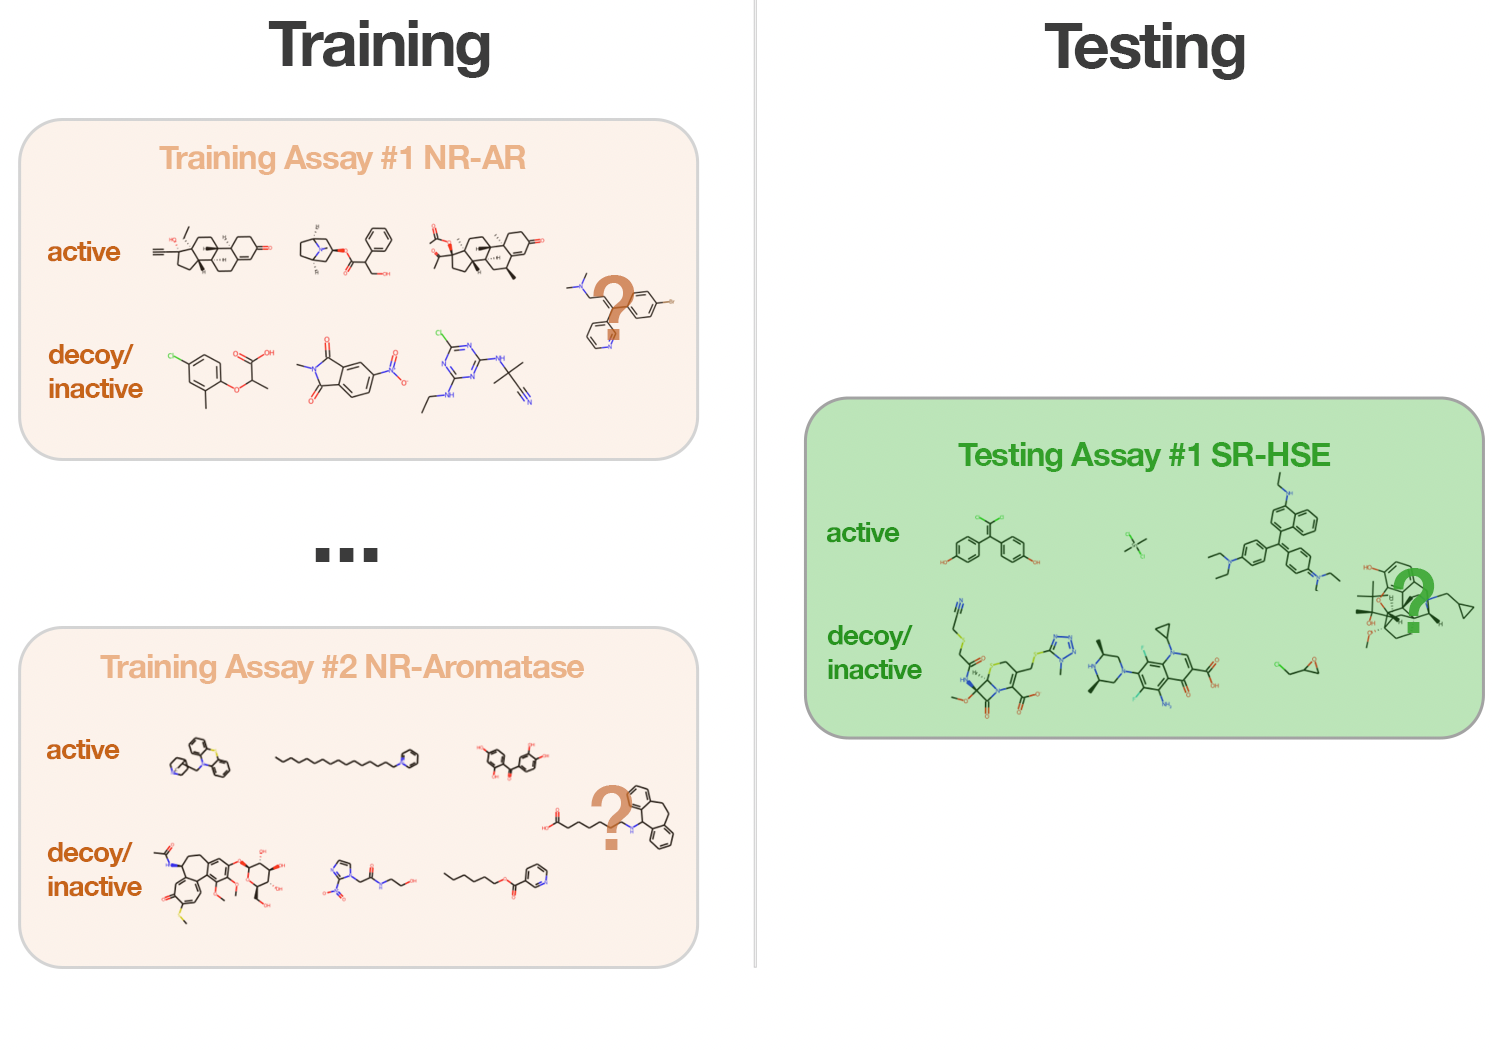
\includegraphics[width=0.8\linewidth]{img/tox21-metalearning.png}
    \caption{2-way 3-shot few-shot classification. Training a meta-learner on experimental assays and generalising for an unseen assay in the Tox-21 dataset.}
    \label{fig:tox21metalearning}
\end{figure}

Building on this notion, we explore few-shot learning to address the low-data problem for hit discovery, lead identification and optimisation. The ability of a machine learning model to learn new concepts fast with just a few training examples is invaluable for this domain, where data on active compounds is scarce. Meta-learning aims to achieve generalising capabilities for previously unseen environments during training time. In few-shot classification, a meta-learning paradigm, we train models using a variety of training tasks and optimise classification performance over a distribution of tasks, including unseen ones. Learning consists of a series of episodes, each consisting of an \textit{N}-way \textit{K}-shot classification task, effectively simulating the conditions at testing time. $N$ refers to the number of classes we include per task, while $K$ refers to the number of molecules we sample for each class to make up the support set \cite{snell2017prototypical}. For this study, few-shot learning refers to training with as little as one example per class, referred to as one-shot learning \cite{koch2015siamese, vinyals2016matching}, to a maximum of ten examples per class. During test time, a small support set is sampled from new, previously unseen targets, and the model uses these few data points to generalise query molecules' activity against this new target \cite{vinyals2016matching}. Figure~\ref{fig:tox21metalearning} shows an example of a typical meta-learning scenario on the Tox21 dataset \citep{huang2016tox21challenge}, where data from a set of assays reserved for training are used to train a model. This model is subsequently used to generalise for a previously unseen assay using only a small support set from this new assay. We highlight that few-shot learning in this problem domain differs from other domains, such as computer vision, where a model is trained to recognise new classes. For example, given a few images of a lion, a class unseen during training, as the support set, the model must generalise for new images of a lion. In the domain under study, the challenge is to train a model that can generalise for the behaviour of molecules in experimental assays which are related but not identical to the assays in the training collection, using only a small support set from these new experimental assays. The molecules used during testing can thus be previously seen during training, but only in the context of their activity for different, but related experimental assays. Given a few molecules from new experimental assays, can the model predict the activity of molecules in this new assay using molecular data for different but related targets as training data?

Molecules are complex structures consisting of atoms and bonds which must be somehow represented in computational space. The classical notation of compounds is the empirical formula such as $C_3H_7NO_2$. However, this can refer to alanine, sarcosine, or lactamide as empirical formulae hold no information on a molecule's topology. Molecular representations such as Extended-Connectivity Fingerprints (ECFP) \cite{rogers2010extended}, and graph convolution learned embeddings \cite{duvenaud2015convolutional} embed more information than the empirical formula on the properties of the molecule. This study mainly explores using graphs as embeddings for the low-data machine learning networks.

A graph $G$ is a natural representation of a molecule, where nodes and edges represent atoms and bonds, respectively. When representing molecules, the set of vertices or nodes \textit{V} intuitively refers to atoms within a molecule, while the set of edges \textit{E} refers to the bonds that connect two atoms; such that $\mathcal{G}=(\mathcal{V}, \mathcal{E})$. Graphs are 2D objects, so spatial properties of a molecule, such as bond angles and chirality, are not inherent to the data object but are instead encoded as node or edge attributes \cite{david2020molecular}. Embeddings of molecular graphs, augmented with atom feature information, can be learned using graph convolutional networks (GCNs). Selected properties such as atomic number, atom type, charge, and valences, among others, may be encoded in a node feature vector. \citet{wu2018moleculenet} report that learned embeddings could be of benefit over topological molecular representations such as ECFP.

In this study, we explore the application of several few-shot learning architectures including, in chronological order, Siamese Networks \citep{koch2015siamese}, Matching Networks \citep{vinyals2016matching}, Prototypical Networks \citep{snell2017prototypical}, and Relation Networks \citep{sung2018learning}. This group of architectures all fall under the umbrella of metric-based meta-learning. In our study, we embed molecule representations using GCNs, and then use or learn a distance function over these embeddings. Effectively, metric-based learners seek to learn a relationship between the input embeddings in the task space. 

\section{Related Work}

Several successful research undertakings have exploited the low-data learning paradigm, especially in the computer-vision domain \cite{koch2015siamese, vinyals2016matching, snell2017prototypical, sung2018learning}. Learning from only a few examples is especially important in domains with a paucity of data. This inaccessibility could be attributed to privacy, safety, or ethical issues and other issues such as the time, resources and exorbitant costs associated with data acquisition. Learning with low-data can lead to less expensive data gathering, and reduced computational cost for learning \cite{wang2020generalizing}.

Building on past work in the metric-based meta-learning sphere \cite{vinyals2016matching}, \citet{altae2017low} introduce a deep-learning architecture for few-shot learning in drug discovery, in which they propose the iterative refinement long short-term memory (IterRefLSTM). IterRefLSTM builds on the Matching Networks \cite{vinyals2016matching} by introducing iterative refinement of embeddings using Long-Short Term Memory (LSTM) networks. In our research, we build on the work by \citet{altae2017low} and extend it by applying other successful few-shot learning approaches explored for other domains, such as the computer-vision domain. The authors employ Graph Convolutional Networks (GCN) to learn molecular embeddings, which are then fed into the low-data architectures for classification.

\subsection{Graph Convolutional Networks}

Molecules must be represented in computational space before processing them using few-shot machine learning techniques. \citet{wu2018moleculenet} report that graph-based models outperform conventional machine learning models on most datasets, suggesting that a learned embedding is advantageous over other molecular representations. Building on this rationale, we opt for graph learned molecular representations to embed the input molecules in this study. 

Graph Convolutional Networks (GCNs) may be used to learn molecular representations \cite{jiang2021could}. Embeddings learned through neural networks afford the construction of automated features rather than fixed fingerprints. GCNs transform small molecules into real-valued vector representations, which are an effective way of processing small molecules via deep neural networks \cite{gomez2018automatic}. \citet{duvenaud2015convolutional} report that using a differentiable method reduces collisions of substructures, and the learned embedding can be optimised to contain relevant features such as biological activity and substructure information.

If the graph object is our input signal, we can apply a set of operators to approximate the function we are attempting to learn. \citet{bronstein2021geometric} propose four key building blocks for deep learning on graphs, which include linear set equivariant layers, non-linear functions, local pooling layers, and set invariant layers. For graphs, the nodes $v$ are found on a domain $\Omega$ such that $v \in \Omega$. The nodes in $\Omega$ are stored in a feature space $C$, such that $C = \mathbb{R}^k$. Using a set of feature functions $X(\Omega, C)$, we can transform the feature space of the nodes in our domain. 

In the equivariant layer $B$, we can take the nodes in our domain and apply a function that transforms the features of the nodes such that $X(\Omega, C) \rightarrow X(\Omega', C')$. Equivariance allows for a function $g$ to be applied before or after this layer, such that $B(g.x) = g.B(x)$. The non-linear activation functions can be applied element-wise on the features of the nodes in a graph, such that $(\sigma(x))(v) = \sigma(x(v))$. Local pooling layers can be used to apply coarsening to the graph such that $X(\Omega, C) \rightarrow X(\Omega', C)$, in which we can reduce the number of nodes in our domain such that $\Omega' \subseteq \Omega$. Finally, we have the invariant layer $Z$, which can also be referred to as a global pooling layer, in which $X(\Omega, C) \rightarrow y$, which satisfies the invariant condition such that $Z(g.x) = Z(x)$ \citep{bronstein2021geometric}. 

% Figure \ref{fig:neuralgraphfingerprint} illustrates an example of a GCN to learn a molecular embedding.

% \begin{figure}[h]
%     \centering
%     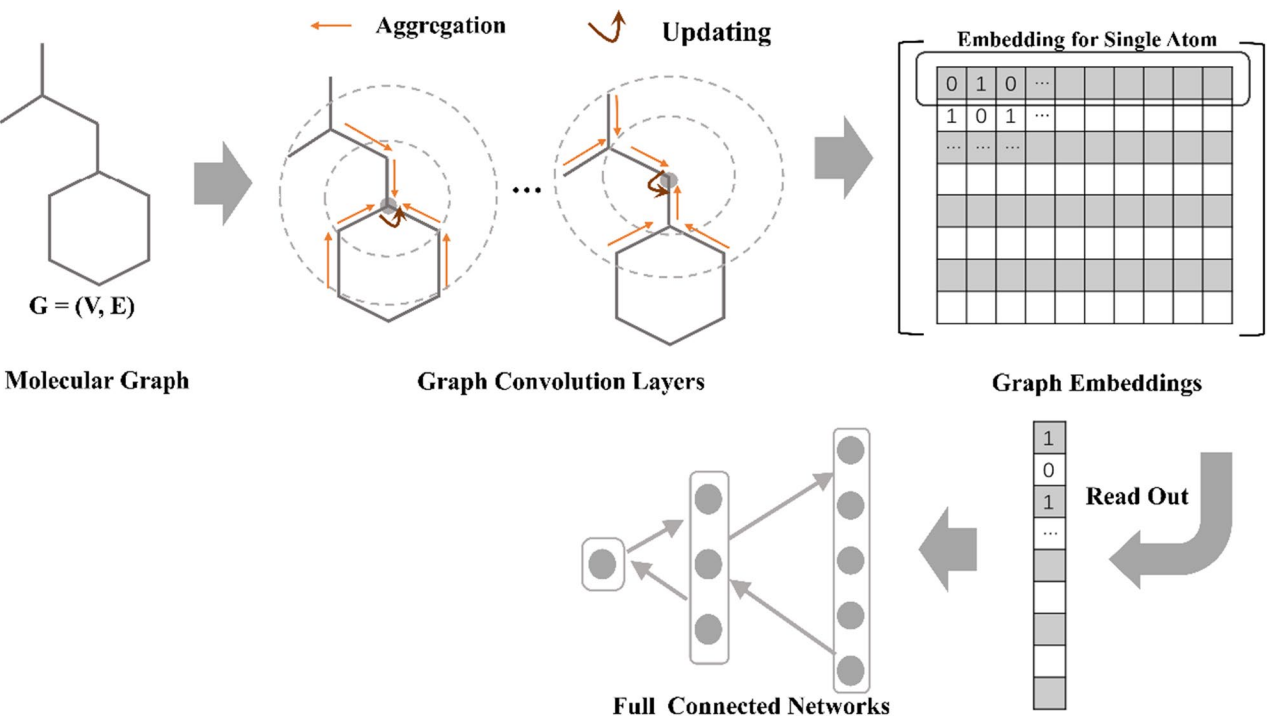
\includegraphics[width=0.9\linewidth]{img/graph_mol_embedding.png}
%     \caption[Learned Embedding through a GCN]{A typical pipeline for representing molecules using a learned embedding function, which can be processed further using feedforward neural networks as shown. Reproduced from \citet{jiang2021could}.}
%     \label{fig:neuralgraphfingerprint}
%   \end{figure}

\subsection{Metric-based Few-Shot Learning}

The success of a few-shot learning model for metric-based meta-learning is dependent on the effectiveness of a kernel $k_\theta$, which measures the similarity between data samples ${x..x_i}$ from a support set $S$ (see Equation \ref{kernel}) using a metric or distance function. The techniques employed in this study, excluding the benchmark model, use the support and query embeddings generated from the GCNs to learn the kernel function. We explore four few-shot learning models in this study, which are presented in the Methodology section. These include Siamese Networks, Matching Networks (upon which the state-of-the-art is developed), Prototypical Networks and Relation Networks. The two latter networks are new approaches for this problem domain and are mostly inspired by the computer vision domain.

\begin{equation}
    \label{kernel}
    P_\theta(y \vert \mathbf{x}, S) = \sum_{(\mathbf{x}_i, y_i) \in S} k_\theta(\mathbf{x}, \mathbf{x}_i)y_i
\end{equation}

\subsubsection{Siamese Networks}

Siamese networks \citep{koch2015siamese} are composed of two identical networks with shared weights and parameters, taking in a pair of data samples (molecules) as inputs. The distance between outputs from each component in the pair of networks is calculated to learn their relationship. The process for learning a classifier using Siamese Networks is visualised in Figure \ref{fig:siamesenetarchi} and is described as follows;

\begin{figure}[h]
    \centering
    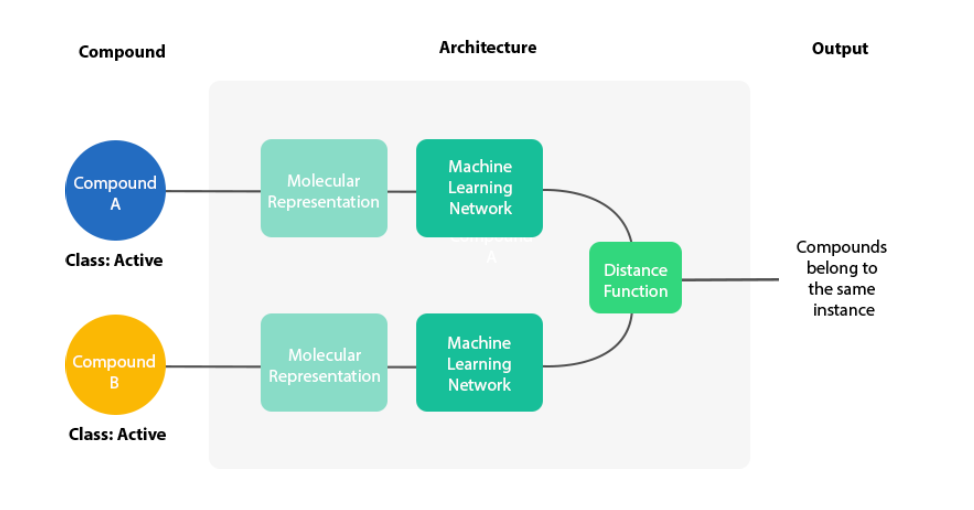
\includegraphics[width=0.9\linewidth]{img/high-level siamese.png}
    \caption[High-level schematic of Siamese network]{High-level schematic of a Siamese network for the molecular network.}
    \label{fig:siamesenetarchi}
\end{figure}

\begin{enumerate}
    \item Generate a list of all possible pairs between training data. If both data samples in the pair have the same target, the pair's label is set to one and zero if otherwise.
    \item Create a twin network using the GCN architecture to embed two molecular graph inputs into latent space.
    \item Calculate the L1 distance between the molecule embeddings. 
    \item The distance between the two embeddings is passed through a linear feedforward layer, followed by a sigmoid function to output the probability that the two molecules belong to the same class.
    \item The binary cross-entropy loss is calculated and backpropagated through the network.
\end{enumerate}

\subsubsection{Matching Networks}

The Matching Networks architecture builds on Siamese Networks. However, instead of learning a metric function over data pairs, the classifier learns how to define a probability distribution of output labels from query examples using a support set $S$. The classifier outputs a sum of attention-weighted labels from the support set to predict the similarity between the query and the support set samples. We use the same embedding function for the support and query sets to compute the molecular embeddings. Subsequently, the cosine similarity of pairs of data points between the support and query sets is computed, which is then normalised by a softmax function. The attention mechanism $a$ in $\hat{y} = \sum_{i=1}^{n} a(\hat{x}, x_i)y_i$ specifies how similar $\hat{x}$ is to each example $x$ in $S$.

\begin{figure}[!ht]
    \centering
    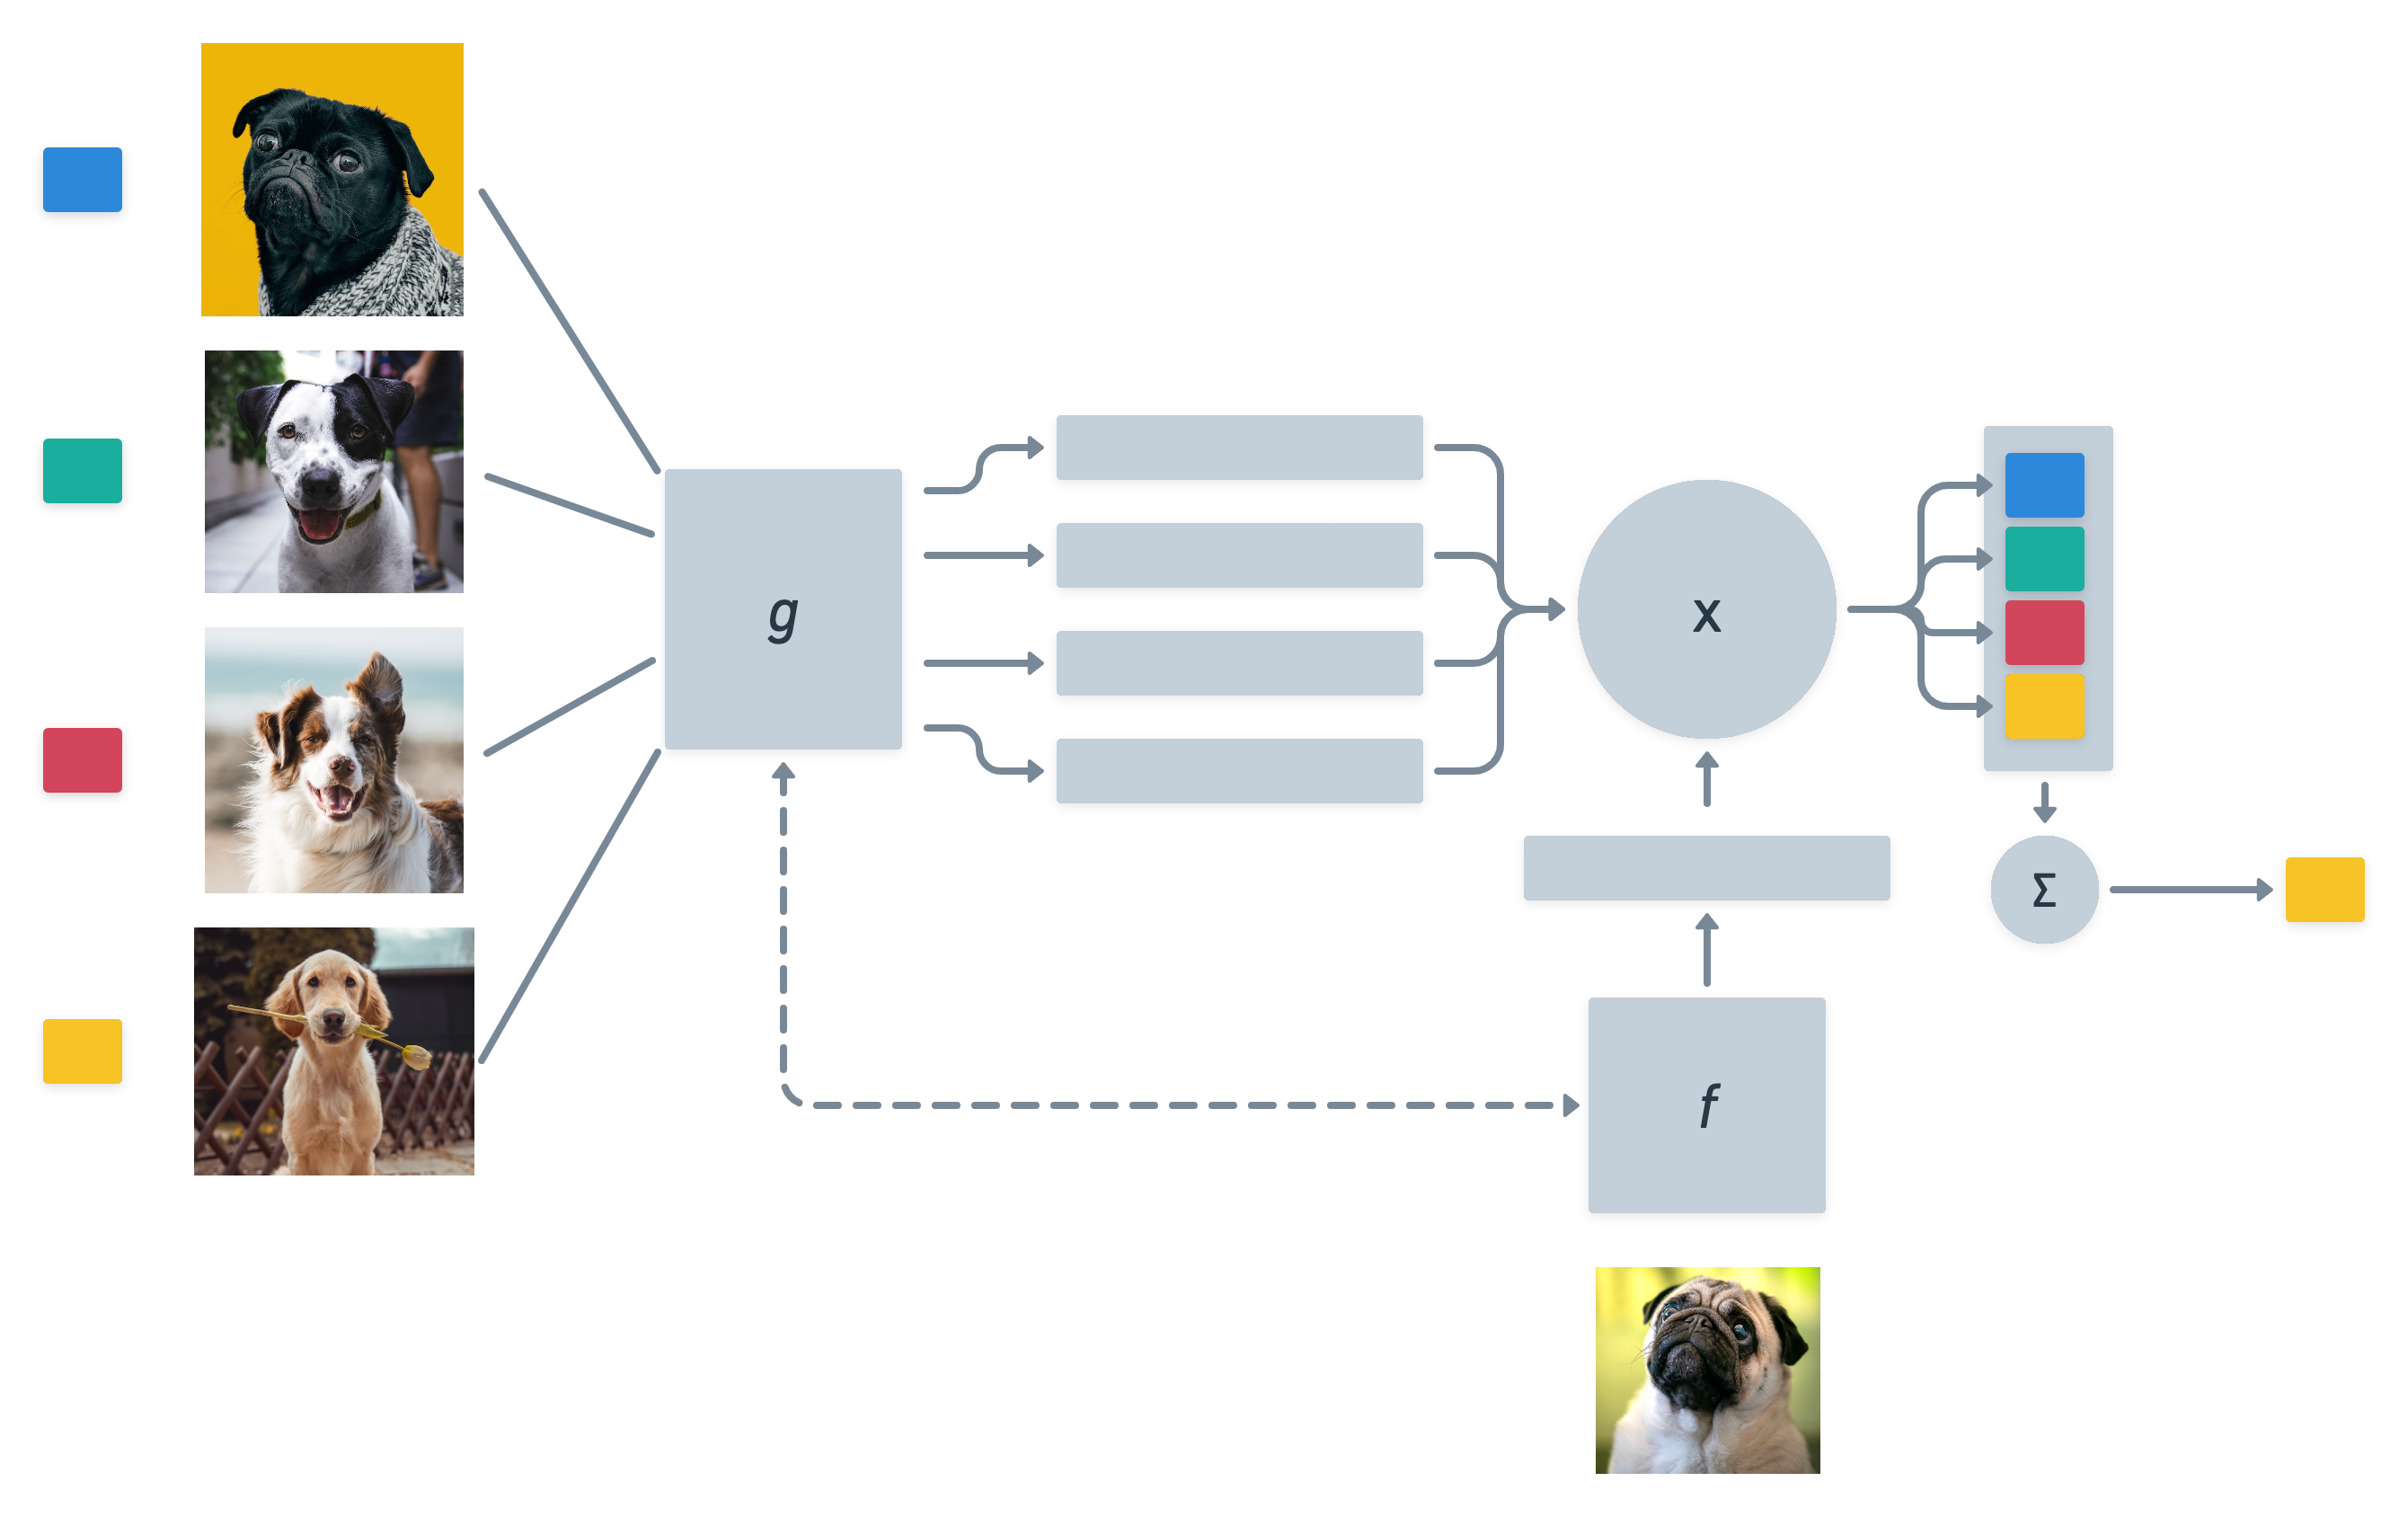
\includegraphics[width=0.7\linewidth]{img/matching_networks_adapt.png}
    \caption[Matching Networks Architecture]{Matching Networks Architecture. Adapted from \citet{vinyals2016matching}.}
    \label{fig:matchingnets}
\end{figure}

Figure~\ref{fig:matchingnets} illustrates the Matching Nets architecture. Embedding functions $f$ and $g$ are Convolutional Neural Networks (CNNs) \citep{lecun1995convolutional}, potentially being identical to each other, which project the inputs to the feature space. \citet{vinyals2016matching} also propose full context embedding functions, which take as input the whole support set with the element $x_i$, thus resulting in \( g(x_i, S) \). Full context embeddings effectively modify how the element is embedded with respect to the whole support set $S$. A bidirectional LSTM is used to encode $x_i$ in the context of the support set. Finally, the attention mechanism $a$, is the classifier which takes a softmax over the cosine distance of the embeddings. As proposed in \citet{vinyals2016matching}, fully contextual embeddings (FCE) are used in our implementation. Taking single data points to learn an embedding function limits the ability to embed the molecules effectively into latent space. Therefore, a bidirectional long-short term memory (LSTM) is used, which takes the whole support set as input to adjust the embedding based on the other support samples. $g_\theta(x_i, S)$ encodes $x_i$, a data sample from the support set, in the context of the whole support set $S$. The LSTM transforms our support set embeddings by adding the forward and backward activations to the original support image embeddings. Subsequently, $f_\theta(x, S)$, encodes the query sample $x$ and trains the LSTM with read attention over the support set. The hidden state is updated over ten processing ``read'' steps until, eventually, the hidden state is equivalent to the aforementioned $f_\theta(x, S)$. The hidden state and the output from the attention function are updated in each iteration. The cross-entropy loss is computed for each query prediction whilst training the model using stochastic gradient descent.

\subsubsection{Prototypical Networks}

Prototypical Networks \citep{snell2017prototypical} have similarities to Matching Networks, but instead of considering the individual support set embeddings, the mean vector of the embeddings (referred to as the \textit{prototype}) for each class within the support set is taken. Another improvement \citet{snell2017prototypical} make over Matching Networks is using Euclidean distance rather than the cosine distance to calculate the distances to classify the query (refer to Figure~\ref{fig:protonets}). In order to classify query data samples, the softmax of the Euclidean distance's inverse between each query and each prototype is taken. The negative log-likelihood is used to train the network through stochastic gradient descent

\begin{figure}[!ht]
    \centering
    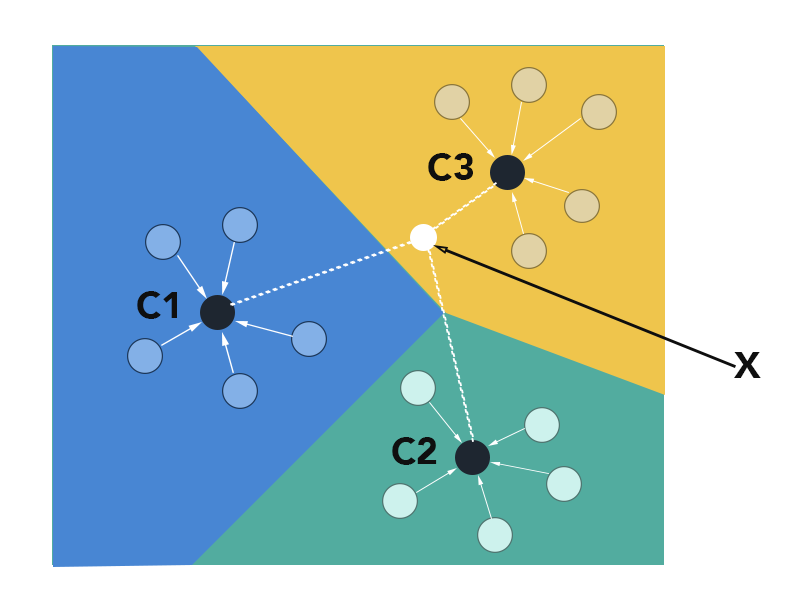
\includegraphics[width=0.7\linewidth]{img/ProtoNetsAdapt.png}
    \caption{Few-shot learning in Prototypical Networks, where prototypes \textbf{$c_k$} are taken as the mean of embedded support examples for each class. Adapted from \citet{snell2017prototypical}.}
    \label{fig:protonets}
\end{figure}

\subsubsection{Relation Networks}

\citet{sung2018learning} present the Relation Network, a framework for few-shot learning but one which could also be extended to zero-shot learning. The Relation Network learns a non-linear distance metric to compare support and query examples. Unlike previously mentioned networks, this network uses a feedforward neural network to learn a distance function in feature space. After embedding the support and query examples using an embedding function, each query example is concatenated with each feature map from the support set. The relationship between the queries and the different classes within the support set is captured by passing the feature map concatenations through a feed-forward neural network $g_\theta([x_i, x_j])$ to predict a relation score. The output class can be inferred from this relation score vector. $[\cdot,\cdot]$ is the concatenation between each support set data sample $x_i$ and the query data samples $x_j$. The Mean Squared Error (MSE) is used as the loss function, as proposed in the original paper. Figure \ref{fig:relationnets} illustrates the Relation Network architecture.

\begin{figure}[h]
    \centering
    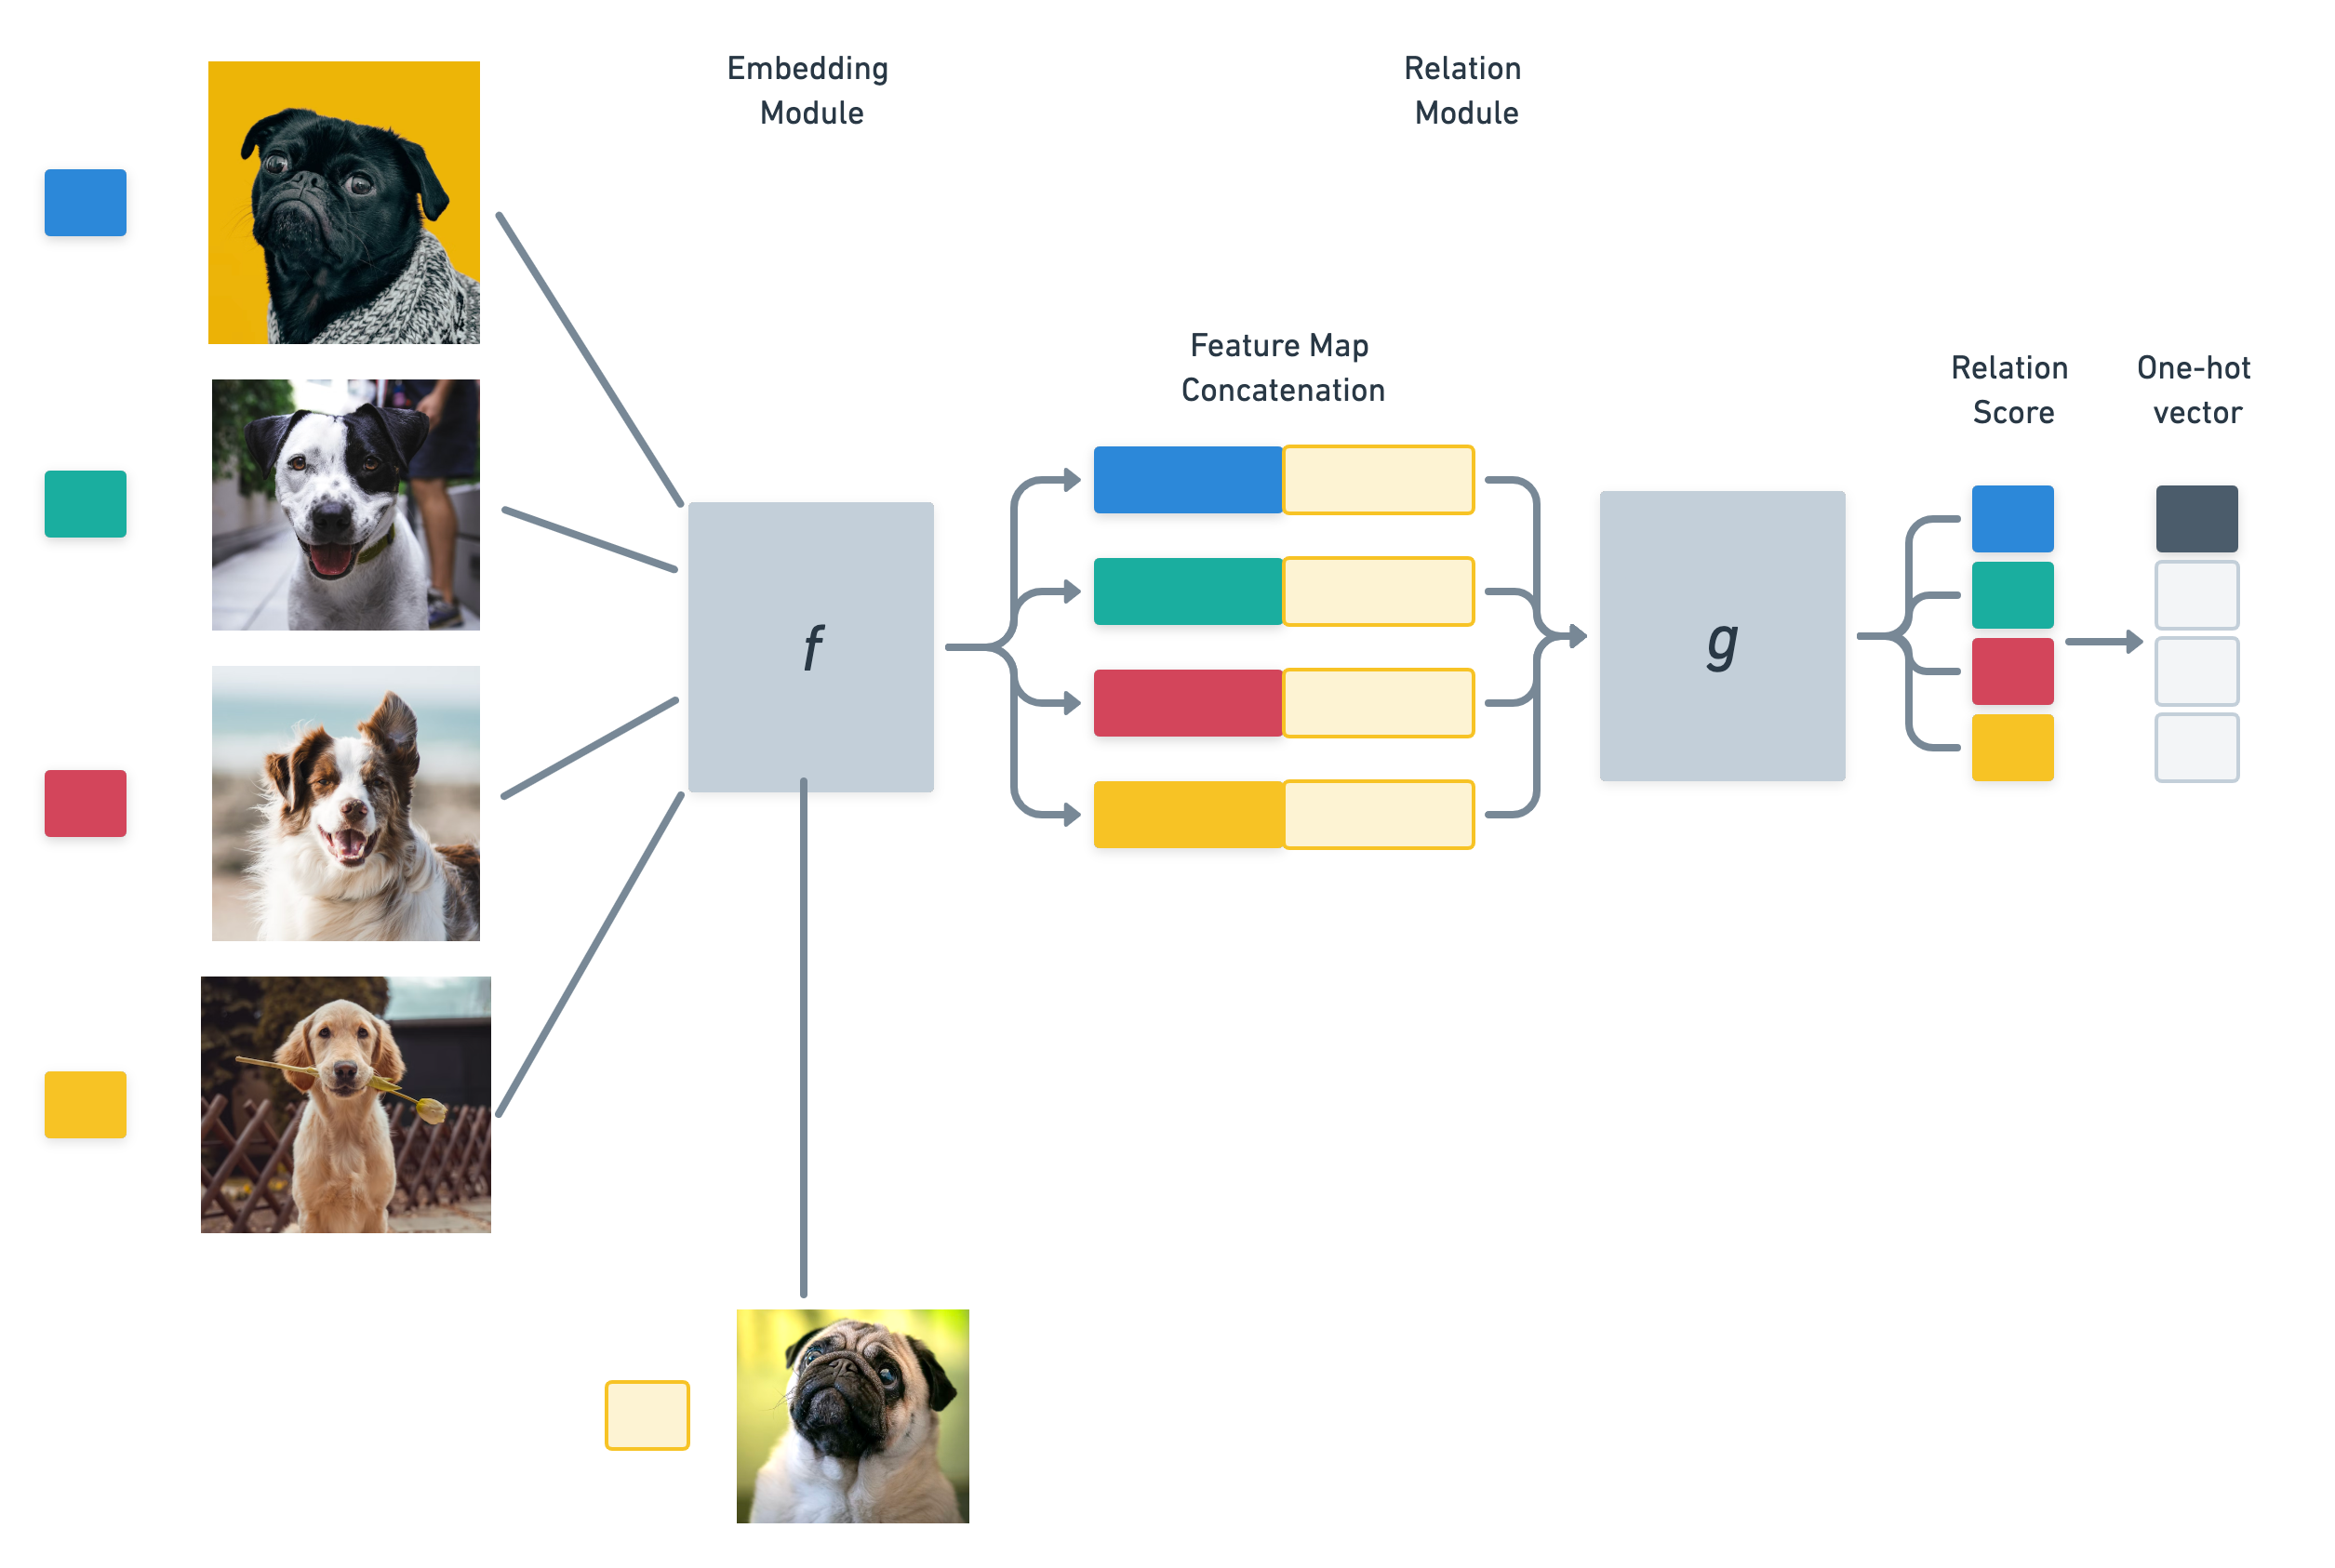
\includegraphics[width=0.9\linewidth]{img/RelationNetAdapt.png}
    \caption[Relation Networks]{Few-shot learning scenario in Relation Networks for a 4-way 1-shot learning task with one query as an example. Adapted from \citet{sung2018learning}.}
    \label{fig:relationnets}
\end{figure}

\subsection{Iterative Refinement LSTM}

\citet{altae2017low} build on meta-learning concepts by training machine learning models on molecular data from a set of experimental assay targets (from the Tox21, SIDER, and MUV datasets) reserved for training. The model is then used to generalise for the activity of molecules in new, previously unseen experimental assays using only a small support set from these new assays. These test assays are related but not identical to the ones reserved for training. The number of molecules sampled for each class in the support set ranges from one to a maximum of ten molecules. The support and query molecules are embedded in their work using a graph convolutional network. Bond information and distinction between bond types was not considered in their study. We note that the \textit{pool} layers do not coarsen the graphs but only apply a max function over neighbouring nodes.

\citet{altae2017low} propose the iterative refinement long-short term memory (IterRefLSTM) to further process the resulting embeddings in a few-shot machine learning pipeline. In IterRefLSTMs two embedding functions $f(\dot|S)$ and $g(\dot|S)$ are developed simultaneously. Therefore, the query embedding is built iteratively with that of the support set, using information from the two sets to enhance both the support and query embeddings. Once the embeddings have been iteratively refined, the authors apply a metric-based function to classify the queries using the support set embeddings. To emulate the Matching Networks, the authors use the Cosine distance to compare embeddings. Figure \ref{fig:schematiconeshotdrug}\footnote{Accessed from: https://pubs.acs.org/doi/10.1021/acscentsci.6b00367 - Further permissions related to the material excerpted should be directed to the ACS.} illustrates a one-shot learning scenario encapsulating the concepts mentioned earlier.

\begin{figure}[h]
    \centering
    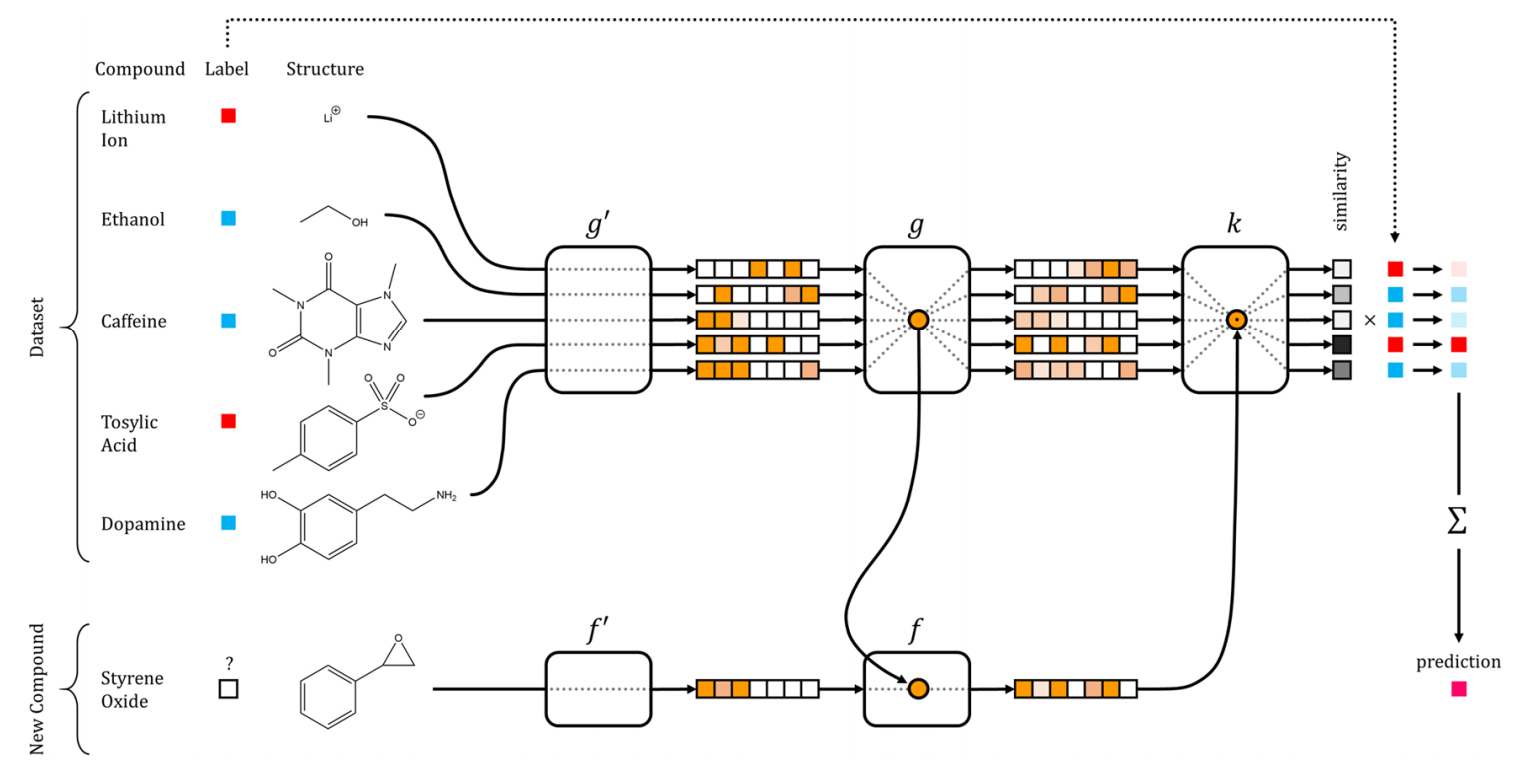
\includegraphics[width=0.9\linewidth]{img/pandeschematic.png}
    \caption[Schematic of one-shot learning in drug discovery]{Schematic of one-shot learning in drug discovery based on the Matching Network \citep{vinyals2016matching} architecture. Reproduced from \citet{altae2017low}.}
    \label{fig:schematiconeshotdrug}
\end{figure}

Their work is evaluated on the Tox21, the Side Effect Resource (SIDER) \citep{kuhn2016sider}, and MUV datasets\citep{rohrer2009maximum}. For every dataset, a subset of the targets is reserved for training and the rest for testing. Training is carried out as explained in the Matching Networks paper, in which training conditions match those at test time \citep{vinyals2016matching}. The authors use a Random Forest (RF) with 100 decision trees as a machine learning baseline model. They also utilise a conventional Graph Convolutional Networks (GCN) \citep{kipf2016semi} as an additional baseline model, which is trained using only a small support set from the test targets. They then experiment with Siamese Networks \citep{koch2015siamese}, Matching Networks \citep{vinyals2016matching}, and an adaptation of the Matching Networks by applying the iterative refinement concepts explained earlier.

The authors utilise ROC-AUC scores to report the performance of the models. Considering the extreme imbalance of the data in the utilised datasets, favouring the negative (inactive/decoy) class, we note that the PR-AUC score would be a more appropriate evaluation measure. PR-AUC is based on the relationship between precision and recall, providing a clearer picture of how the model performs when predicting the \textit{positive} (active) class in the data. Correctly predicting the ``active'' class is of significant importance in virtual screening.

On the Tox21 and SIDER datasets, their proposed machine learning architecture achieves good ROC-AUC performance. The mean score for 10-shot learning on the median held-out task on Tox21 achieves a score of $0.823 \pm 0.002$, while for one-shot learning, the model achieves a mean score of $0.827 \pm 0.001$. The reasons why one-shot learning achieved better performance than 10-shot learning is uncertain, as we expect the model to perform better with larger support sets. However, this might be attributed to variance in the data between experiments. On MUV data, the baseline machine learning models performed few-shot learning. The authors report that this is due to MUV data being maximally informative; therefore, structural similarity cannot be utilised to generalise activity prediction. The authors open-sourced their models in the DeepChem library\citep{ramsundar2019deep}. However, the implementations are now outdated and we were unable to train and test these models using the provided scripts. However, we study the open-sourced implementation and the respective details in the original literature to reproduce their work successfully.

\section{Methodology}


In this work, we implement a Random Forest and a Graph Convolutional Network (GCN) to use as benchmark models. Additionally, we implement four few-shot machine learning architectures, namely, Siamese Networks, Matching Networks, Prototypical Networks, and Relation Networks. The state of the art, IterRefLSTMs \citep{altae2017low}, are used to enrich the resulting embeddings in latent space. Molecules are represented as graph objects, which are then processed using GCNs to produce a vectorised embedding in computational space. Throughout our work, we try to follow the implementation of \citet{altae2017low} as closely as possible for the sake of reproducibility and homogenising the results for comparison.

%% TODO @@ DV seven steps text + FIGURE... 

\subsection{Datasets}

In this work, we make use of the following three datasets;

\begin{itemize}
    
    \item \textbf{Tox21} \citep{huang2016tox21challenge} -- Mainly used for lead optimisation, containing toxicity data for 12 targets \citep{tox21}. The dataset was obtained from the DeepChem AWS bucket\footnote{Accessed from: \url{https://deepchemdata.s3-us-west-1.amazonaws.com/datasets/tox21.csv.gz}. Last Accessed: 26/05/2022} in CSV format. The NR-AR, NR-AR-LBD, NR-AhR, NR-Aromatase, NR-ER, NR-ER-LBD, NR-PPAR-gamma, SR-ARE, SR-ATAD5 targets are reserved for training, and the remaining SR-HSE, SR-MMP, SR-p53 targets are used for testing.
    
    \item \textbf{Maximum Unbiased Validation (MUV)} \citep{rohrer2009maximum} -- Based on PubChem BioAssays, used for validating virtual screening techniques against 17 different targets \citep{rohrer2009maximum}. The dataset was obtained from the DeepChem AWS bucket\footnote{Accessed from: \url{https://deepchemdata.s3-us-west-1.amazonaws.com/datasets/muv.csv.gz}. Last Accessed: 26/05/2022} in CSV format. A total of 12 targets (MUV-466, MUV-548, MUV-600, MUV-644, MUV-652, MUV-689, MUV-692, MUV-712, MUV-713, MUV-733, MUV-737, and MUV-810) are reserved for training, while MUV-832, MUV-846, MUV-852, MUV-858, and MUV-859 are reserved for testing.
    
    \item \textbf{Directory of Useful Decoys (Enhanced) (DUD-E)} \cite{mysinger2012directory} -- Used for benchmarking virtual screening techniques by introducing a number of active compounds against specific targets. For each active, a number of \textit{decoys} with similar physical properties, but different topologies, are made available. For this research study, we made use of the GPCR subset of the DUD-E dataset \citep{mysinger2012directory}. The data was obtained directly from the DUD-E website.\footnote{Accessed from: \url{http://dude.docking.org/subsets/gpcr}. Last Accessed: 26/11/2022} The AA2AR, DRD3, and ADRB1 targets are used for training. Two targets, ADRB2 and CXCR4, are reserved for testing.
\end{itemize}

Table~\ref{table:datasetimbalance} shows the excessive imbalance of these datasets, highlighting the scarceness of data on active compounds in this domain. Due to this class imbalance we select appropriate performance metrics (see Evaluation Section).

\begin{table}[h]
	\centering
	\caption{Number of actives and inactives/decoys across all targets in the datasets used. Figures in parentheses show the percentage of the total compounds in the dataset.}
	\begin{tabular}{@{}crr@{}}
		\hline
		Dataset 		& Actives 			& Inactives/Decoys \\
		\hline
		Tox21 			& 4,149 (7.04\%) 	& 54,746 (92.96\%) \\
		MUV 			& 347 (0.20\%) 		& 175,990 (99.80\%) \\
		DUD-E (GPCR) 	& 1,249 (1.45\%) 	& 84,856 (98.55\%) \\
		\hline				
	\end{tabular}
	\label{table:datasetimbalance}
\end{table}



\subsection{Molecular Representations}

We first standardise the molecules according to a set of well-defined and consistent rules and conventions. It is of utmost importance to maintain uniformity and integrity across the different datasets (and sources) being used. \citet{bento2020open} present an open source chemical structure curation pipeline based on RDKit\citep{rdkit} for validating and standardising chemical structures, which follow FDA/IUPAC guidelines \citep{brecher2006graphical, food2007substance}. Their work is available in the ChEMBL Structure Pipeline package \cite{bento2020open} and is used to standardise the molecules in our pipeline. 

We create a molecular graph from the SMILES string of the standardized molecule using RDKit, an open-source toolkit for cheminformatics. We then one-hot encode eight features for the atoms in each molecule, namely, atom type, atomic number, atom degree, explicit valence, hybridisation, formal charge, number of radical electrons, and aromaticity. Self loops are added to every node in the generated graph, so aggregation functions during message passing consider the features of the node itself. The order of the atoms follows the canonical order of the atoms assigned through RDKit. We make use of the Deep Graph Library (DGL) LifeSci \cite{dgllife} library to create the graph objects and subsequently process them using the DGL library \cite{wang2019dgl}.



\subsection{Episodic Learning}

Figure~\ref{fig:episodiclearning} illustrates a high-level overview of the episodic learning methodology. Training for few-shot learning is carried out in a series of episodes, framed as \textit{N-way K-shot} classification tasks. We consider \textit{N-way K-shot} classification tasks, where the support set contains \textit{N} classes and \textit{K} labelled molecules. These classification tasks match the conditions at training time with those during testing, as proposed by \citet{vinyals2016matching}. The tasks in our research are binary classification tasks, therefore \textit{N} is always set to two to represent the active and the inactive/decoy class respectively. Experiments with varying values of \textit{K} are carried out to generate the support sets, with a minimum of one data point, to a maximum of ten data points (molecules) per class. The combinations for \textit{K} active and inactive/decoy classes are not exhaustive, but we follow the support set composition used in \citet{altae2017low} to directly compare results with this study.

\begin{figure}[ht!]
	\centering
	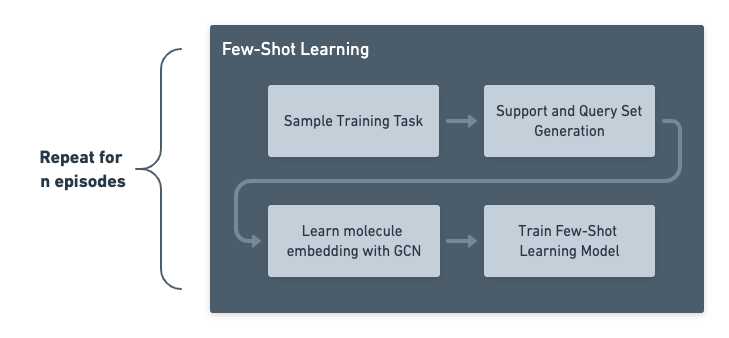
\includegraphics[width=0.9\linewidth]{img/episodic-learning.png}
	\caption{Episodic learning schematic}
	\label{fig:episodiclearning}
\end{figure}

Table~\ref{table:support-set-sizes} contains the composition of the support sets used in our experiments. For each episode, we sample a total of 128 query molecules, which is composed of a balanced combination of molecules from each class. If the active class for a specific target contains less than 64 molecules, the active molecules are over-sampled such that each query set contains 64 actives. The choice of the support set composition was based on the methodology presented in \citet{altae2017low}.

\begin{table}
	\centering
	\begin{tabular}{@{}rrr@{}}
		\hline
		Actives & Inactives/Decoys & Support Set Size \\
		\hline
		10  & 10 & 20 \\
		5   & 10 & 15 \\
		1   & 10 & 11 \\
		1   & 5  & 6 \\
		1   & 1  & 2 \\
		\hline
	\end{tabular}
	\caption{Support set composition}
	\label{table:support-set-sizes}
\end{table}



\subsection{Machine Learning Models}

Before processing the molecular graph, the model first learns an embedding using graph neural networks. Four different architectures, including Siamese, Matching, Prototypical and Relation Networks, process the learned graph embeddings to train our meta-learner. IterRefLSTMs are utilised to refine the latent space embeddings. 

\begin{figure}[ht!]
	\centering
	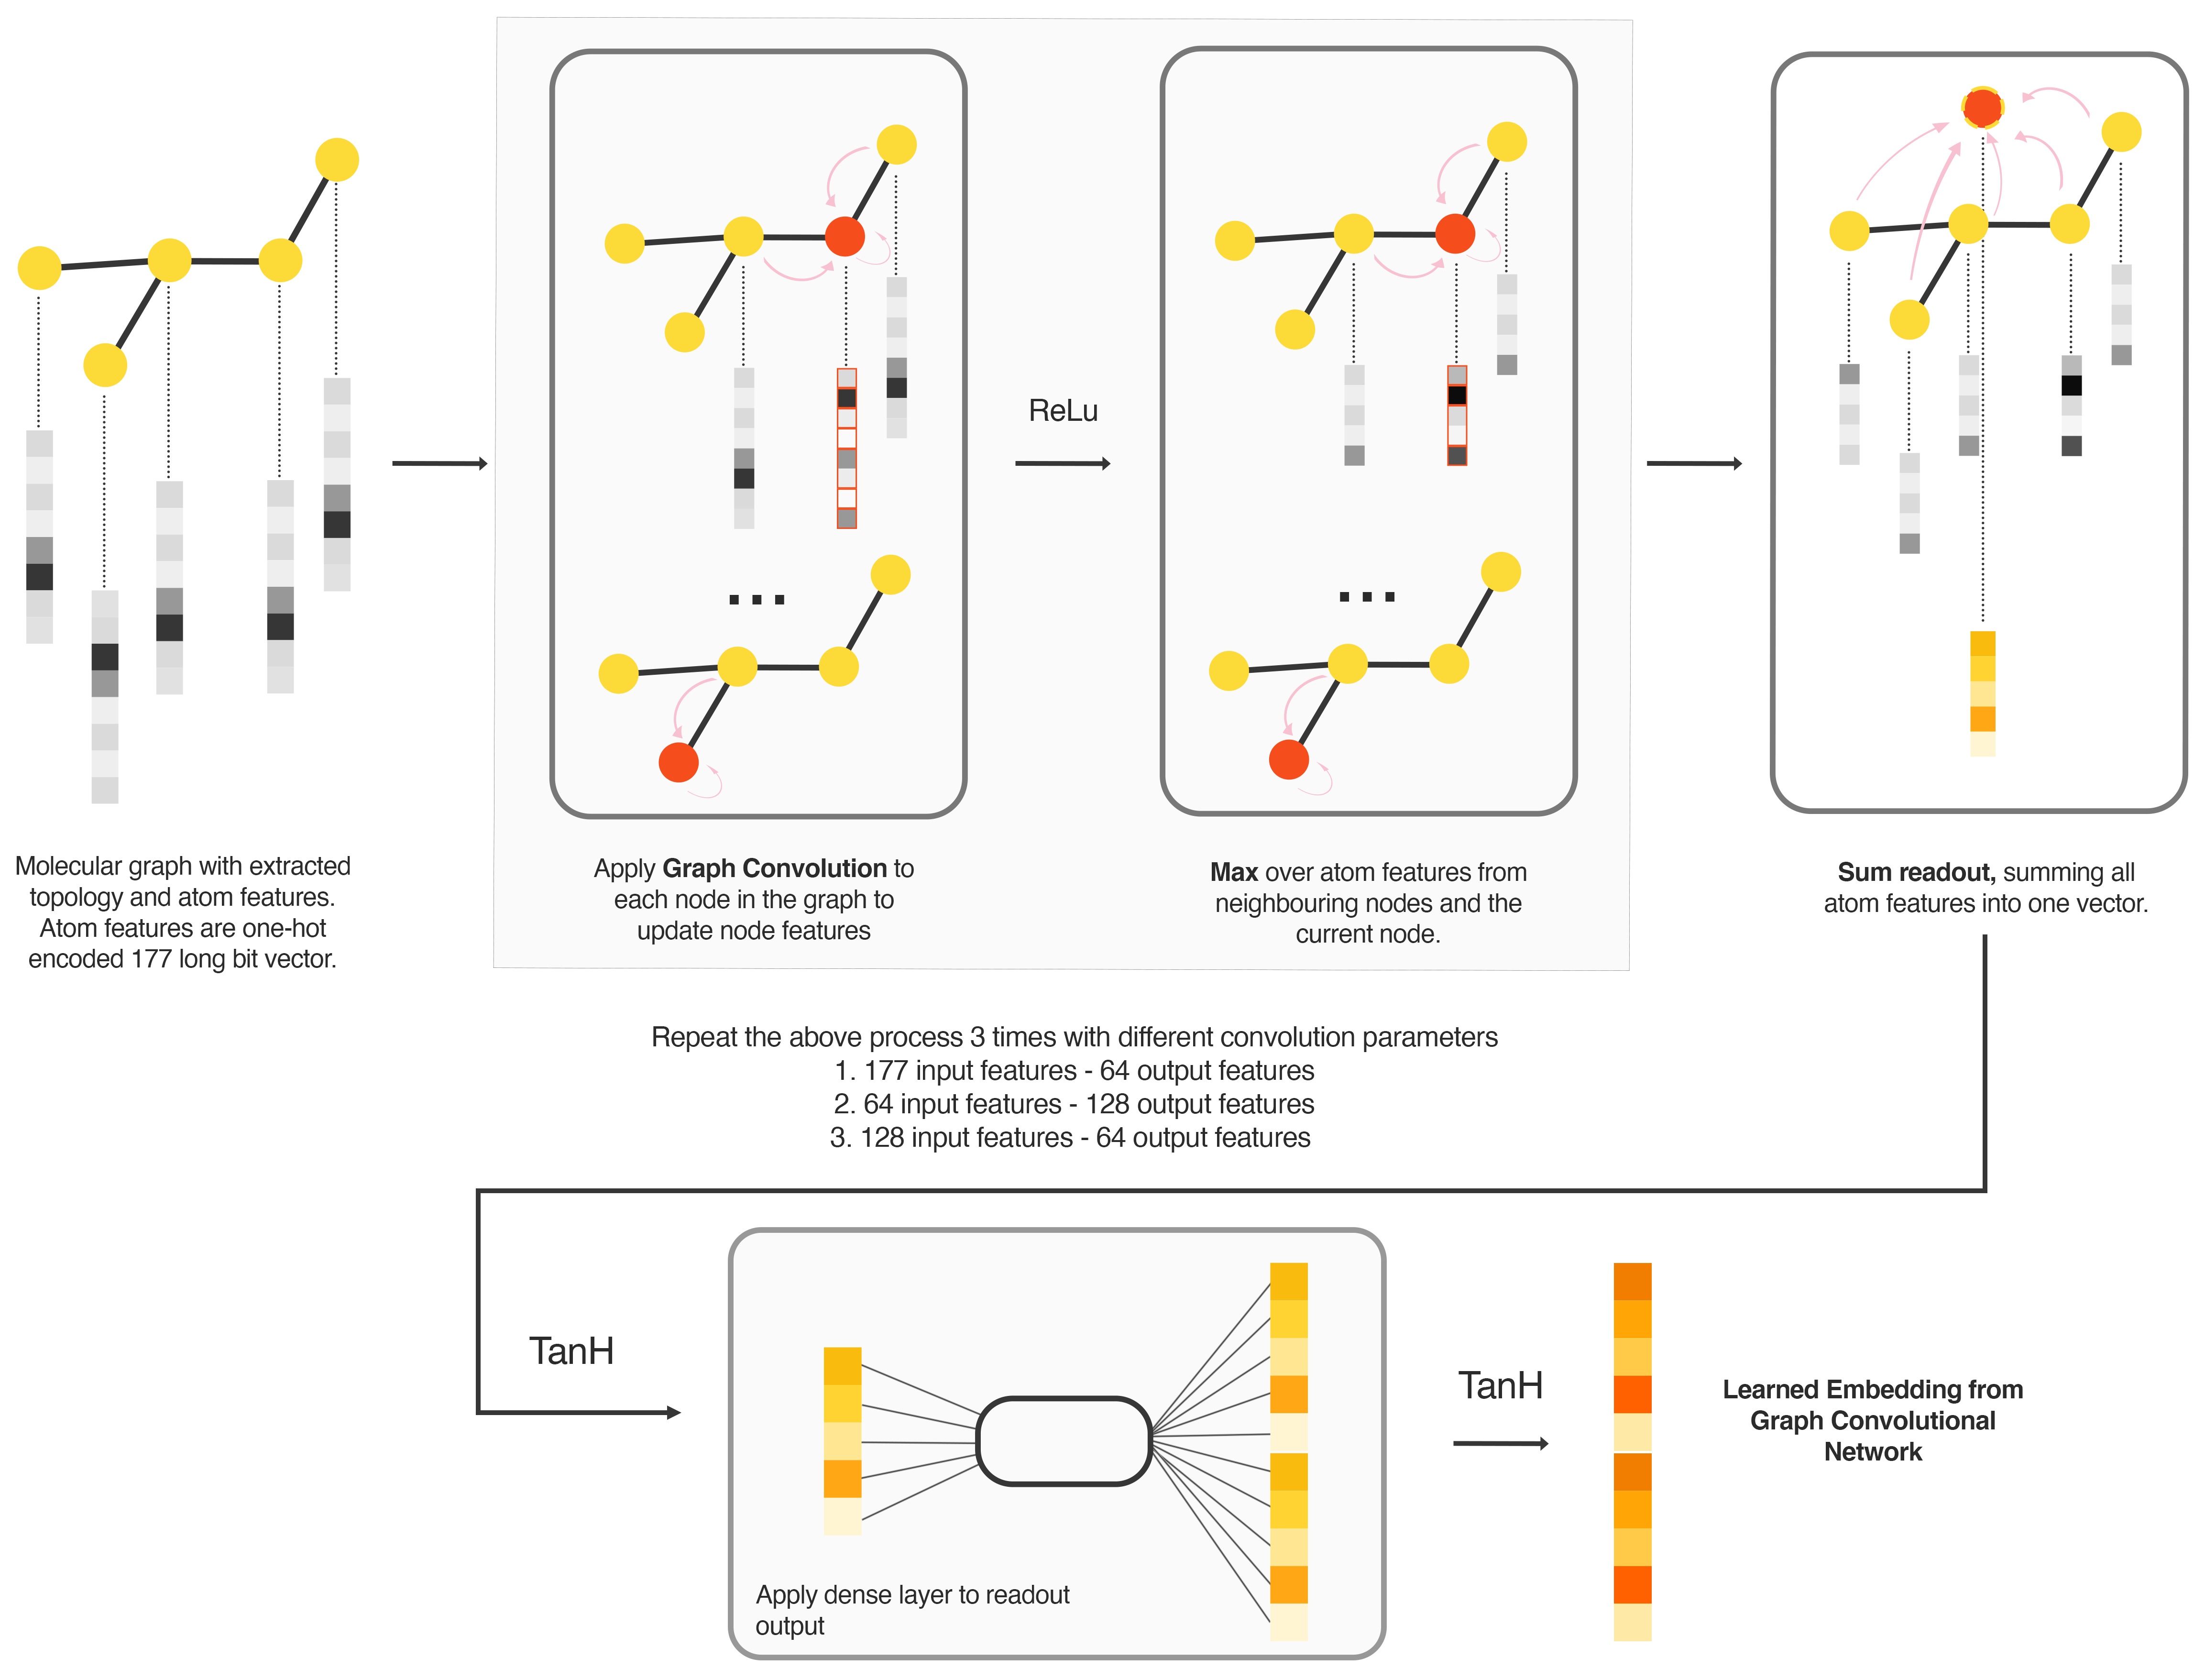
\includegraphics[width=0.75\textwidth]{img/DVGCNArchi.png}
	\caption{Learning an embedding through a Graph Convolutional Network (GCN). The molecule, represented as a graph object with nodes, edges, and atom features, is processed using graph convolutions. A max message-passing function over the current and neighbouring nodes follows each convolution layer. After this process, a sum readout aggregates all atom features into one vector. A tanh function activates this vector, and a dense linear layer processes the output vector. A non-linear tanh function activates this vector to yield the final learned molecular embedding.}
	\label{fig:dvgcnarchi}
\end{figure}

\subsubsection{Graph Convolutional Networks}

Graph convolutional networks (GCNs) are used to learn embeddings for the support and query molecules in latent space. Figure~\ref{fig:dvgcnarchi} illustrates the GCN pipeline to learn a molecular embedding. In our study, we make use of the convolutional operator from \citet{kipf2016semi} to process graphs and learn the molecular embeddings.

\begin{equation}
	\label{gcnequation2}
	h_i^{(l+1)} = \sigma(b^{(l)} + \sum_{j\in\mathcal{N}(i)}\frac{1}{c_{ji}}h_j^{(l)}W^{(l)})
\end{equation}

The convolutional layer can be mathematically defined through Equation~\ref{gcnequation2}. $h_j$ is the feature set of the node, $N_i$ is the set of neighbouring nodes $i$, $b$ is the learnable bias, and $c_ji$ is the product of the square root of node degrees. From a message-passing perspective, this can be summarised into the following steps for every node feature space $u$;

\begin{enumerate}
	\item Aggregating the neighbouring representations $h_v$, producing an intermediate representation $\hat{h}_u$.
	\item Transforming $\hat{h}_u$ through a linear projection and a non-linearity function such that $h_u = f(W_u \hat{h}_u)$ \citep{kipf2016semi}.
\end{enumerate}

Three convolutional layers are present in our architecture, after which a maximum function aggregating the node features with the maximum value of the neighbours and the node itself is applied. We highlight that this is not a coarsening operation, as the number of nodes remain the same. Finally, we apply a global pooling layer (readout), in which we sum over the node features of every node in the graph (see Equation~\ref{gcnequationsum}). 

\begin{equation}
	\label{gcnequationsum}
	r^{(i)} = \sum_{k=1}^{N_i} x^{(i)}_k
\end{equation}

A linear transformation is applied to the output from the readout layer, followed by a non-linear activation function, for which we use a hyperbolic tangent function (tanh), outputting the final molecule embedding. Table \ref{table:gcn-architecture} contains the architecture utilised for the GCN in this study, and is illustrated in Figure~\ref{fig:dvgcnarchi2}.

\begin{table}
	\centering
	\begin{tabular}{@{}lrrl@{}}
	\hline
	\textbf{Layer Type} & \textbf{Input Dimension} & \textbf{Output Dimension} & \textbf{Non-Linearity} \\
	\hline
	GraphConv & 177 & 64 & ReLU \\
	Max Pooling & 64 & 64 & \\
	GraphConv & 64 & 128 & ReLU \\
	Max Pooling & 128 & 128 & \\
	GraphConv & 128 & 64 & ReLU \\
	Max Pooling & 64 & 64 & \\
	SumPool Readout & 64 & 64 & tanh \\
	Linear & 64 & 128 & tanh \\
	\hline	
	\end{tabular}
	\caption{Graph Convolution Network Architecture}
	\label{table:gcn-architecture}
\end{table}

\begin{figure}
	\centering
	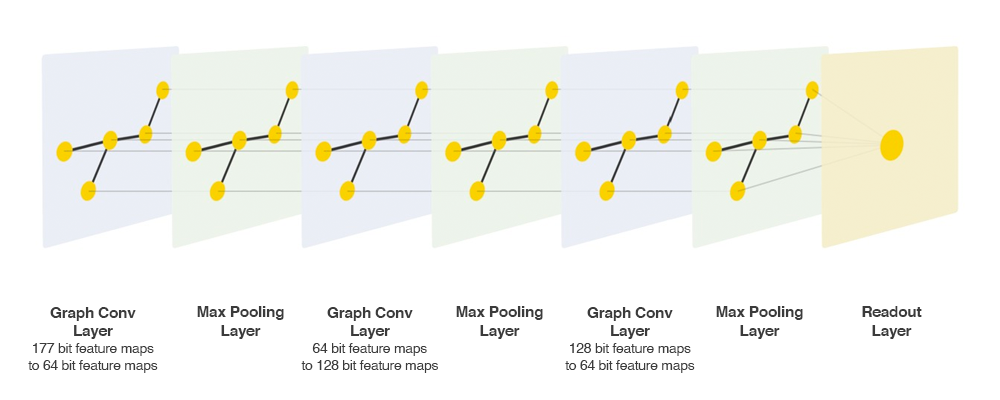
\includegraphics[width=1\linewidth]{img/gcn-layers.png}
	\caption[Layers for graph processing in our GCN.]{Graph processing layers in our GCN implementation. The graph convolution layers apply operations on each individual node's feature maps based on neighbouring nodes. The ReLU function is applied after each convolutional layer, and the tanh function is applied after the final readout layer.}
	\label{fig:dvgcnarchi2}
\end{figure}

\subsubsection{Benchmark Models}

We make use of a Random Forest model with 100 decision trees and a Graph Convolutional Network (GCN) to build a baseline to benchmark the purpose-built few-shot learning models. For the random forest model, ECFP representations of the molecules of size 2,048 bits are used for the classification task, using a radius of two. Meanwhile, the same GCN architecture used for the few-shot learning models is used for our benchmark. The only addition to the architecture is a final linear, fully-connected layer that takes as input 128 features, which is the size of the embedding used for the experiments to follow, and outputs a feature of size one, onto which we apply a non-linear function, in this case a Sigmoid function, to output the probabilities for a binary target (${0, 1}$). This binary target signifies whether the molecule belongs to the active or inactive/decoy class in the experimental assay. These two models are trained on a small support set, sampled from the targets assigned for testing. The remaining data for the designated target is used for testing.

We also carry out a final benchmark test in retrospect by taking a random selection of query molecules from a test target, generating the ECFP with the same aforementioned parameters and then calculating the Tanimoto distance to classify the remaining test molecules based on this distance. However, we find that this does not hold any significant predictive capability. 

\subsubsection{Few-Shot Learning Models}

%% TODO @@ DV to add actual architectures of each of the four models ... and to trim (aggressively) the below since it is repetitive with Episodic Section in the Methodology

Episodic learning is used to train a few-shot machine learning model. \citet{vinyals2016matching} suggest that conditions during training must match those during testing. Training consists of a sequence of learning problems where the model is supplied with a \textit{support} set and a corresponding \textit{query} set. The support set consists of a few molecules sampled from each class, in our case representing the active molecules and the inactives/decoys. We consider \textit{N-way K-shot} classification tasks, where the support set contains \textit{N} classes and \textit{K} labelled molecules. \textit{N} is always assigned a value of two as we are attempting to solve a binary classification problem, whereby the model tries to classify the query molecules as active or inactive in a specific experimental assay. We experimented with a varying number of molecules for the support sets, however the minimum limit was set to one compound per class, while the maximum was set to 10 compounds per class. The \textit{2-way N-shot} formulation is what the model is presented with at test time. We sample a total of 128 query molecules for each episode, which is composed of a balanced combination of molecules from each class. If the active class for a specific target contains less than 64 molecules, the active molecules are over-sampled such that each query set contains 64 actives. We reproduce the work of \citet{altae2017low} from scratch and also apply the IterRefLSTM to the embeddings from all other networks to effectively compare our contribution to past work. Additionally, we also provide implementations for the Prototypical Networks and Relation Networks. All the experiments are run on Google Colaboratory and all implementations are open-sourced on GitHub.\footnote{Accessed From: https://github.com/danielvlla/Few-Shot-Learning-for-Low-Data-Drug-Discovery}

%% -----------------------------------------------------------------

\subsubsection{Evaluation}

The evaluation metrics used in this study are the Area Under Curve (AUC) of the Receiver Operating Characteristic (ROC) curve, and the Precision-Recall Curve (PRC). The state-of-the-art \cite{altae2017low} only reports ROC results, however, this metric alone does not fully encompass the nature of the performance of the machine learning models due to the highly imbalanced nature of the data at hand. In virtual screening, the detection of rare events (equivalent to our minority active class) holds significant importance, as active compounds against a specific target should be identified from the compound database. However, we do not disregard the importance of correct classification of the majority inactive/decoy class, as this is also important for filtering out thousands of screened compounds. As the active class is the minority class, PR-AUC are used to evaluate how well the model can classify the active class. The former is related to a low false negative rate, meaning active compounds incorrectly classified as inactive/decoys, while high precision is attributed by a low false positive rate, meaning compounds classified as active when in fact they are inactive/decoys. The ideal scenario for predicting the minority active class is thus one where we achieve high recall and high precision. Given that the active class is in such a minority, even a small false positive rate could result in high numbers of false positives, due to the high number of the negative class examples. We apply statistical analysis on the ROC and PRC scores from the 20 test rounds for each experiment to establish whether there are significant differences between the few-shot learning models. The scores are compared against those of the model that obtained the best result for the same conditions. Comparison of results between two models is carried out using the Mann-Whitney U-test, also referred to as the Wilcoxon rank sum test \citep{mann1947test}. The tabulated results are the mean values from 20 randomly sampled test rounds, encompassing all the test targets, along with the standard deviation for each mean. The results for each individual target is available in the appendices.

\section{Results}

In this section we present the few-shot model results for the three evaluation datasets, Tox21, MUV, and DUD-E. All these datasets are highly imbalanced, where the inactive/decoys greatly outnumber the number of actives. This defining feature of these datasets presents a challenging problem, but is also further evidence that low-data machine learning is highly beneficial in this domain. We first present the work we reproduced from \citet{altae2017low}, which we also test on a subset of the DUD-E dataset. This was not explored in the original study. The reproduced work includes Siamese Networks \citep{koch2015siamese} and the Matching Networks \citep{vinyals2016matching} with the Iterative Refinement LSTM (IterRefLSTM). The latter obtained the best results in \citet{altae2017low}. This is followed by the presentation and discussion of the results for two newly proposed machine learning models in this domain, which are based on work of \citet{vinyals2016matching} for Matching Networks. These machine learning models include the Prototypical \citep{snell2017prototypical} and Relation \citep{sung2018learning} Networks. Finally, we evaluate the results with the state of the art, which is identified to be the work of \citet{altae2017low}.


\subsection{Tox21}

In line with the results reported by \citet{altae2017low}, the few-shot learning models on Tox21 outperform the benchmark models significantly. The Matching Networks with IterRefLSTM performs well and obtain the best ROC results in a number of experiments. The fact that the same implementation for the Matching Networks (MNs) obtained slightly better results (1-14\% across the five support set experiments) than the state-of-the-art work, can be attributed to the set of atom descriptors used for the initial graph representations presented earlier. Our few-shot learning architecture implementation is identical to the work of \citet{altae2017low}, however variations in how the model learns could be present. Hence, we focus mainly on the performance of how our implementations performed against each other. The results from the Prototypical Networks (PNs) overall outperform the results from the MNs based on statistical analysis (see Table~\ref{table:Tox21-mean}). Meanwhile, MNs and PNs, overall outperform Relation Networks (RNs) in both ROC and PRC performance. 

Results for one shot-learning do not provide a clear-cut choice between our implementations for MNs and PNs with the IterRefLSTM, which is expected due to the architecture of these methods.  In a one-shot learning scenario, MNs and PNs are conceptually similar. The main difference lies in the distance function used as for MNs we use the cosine distance, while for PNs, we make use of the euclidean distance, as proposed in the original literature which introduced these two techniques. They both achieve comparable performance on Tox21 targets for one-shot learning. The performance of MNs for this scenario is consistent with the state-of-the-art work and for such a difficult scenario (i.e.\ learning with only one example from each class), results are promising. The \textit{prototypes} in PNs are a mean of all embeddings for each class in the support set. The euclidean distance between the \textit{prototypes} and each embedding from the query set is calculated to predict the query's activity. As in one-shot learning we only have one example per class, the \textit{prototypes} are equivalent to the embedding for each class, making this identical to the MNs. 

\begin{table}
	\caption{Mean ROC and PRC Scores with standard deviation for ML Models for the Tox21 Test Targets over 20 rounds of testing. Bold text illustrates the best obtained value. The first column shows the composition of the support set. The reproduced results from the model used in \citet{altae2017low} is the MatchingNet.}
	\centering
	% \ra{1.3}
	% {\renewcommand{\arraystretch}{1}}
	\resizebox{\textwidth}{!}{%
		\begin{tabular}{@{}cccccccc@{}}
			\hline
			\textbf{Tox21} & \textbf{Metric} & \textbf{RF} & \textbf{Graph Conv} & \textbf{SiameseNet} & \textbf{MatchingNet} & \textbf{ProtoNet} & \textbf{RelationNet} \\
			\hline
			10+/10- & ROC & 0.617 ± 0.060 & 0.620 ± 0.065 & 0.825 ± 0.043 & 0.824 ± 0.022 & \textbf{0.826 ± 0.034} & 0.814 ± 0.030 \\ & PRC & 0.158 ± 0.102 & 0.150 ± 0.095 & 0.226 ± 0.107 & 0.367 ± 0.105 & \textbf{0.384 ± 0.105} & 0.360 ± 0.102\\
			\hline
			5+/10- & ROC & 0.602 ± 0.059 & 0.610 ± 0.062 & 0.828 ± 0.069 & \textbf{0.824 ± 0.033} & 0.823 ± 0.038 & 0.822 ± 0.023 \\ & PRC & 0.148 ± 0.090 & 0.152 ± 0.094 & 0.190 ± 0.094 & 0.369 ± 0.110 & \textbf{0.388 ± 0.111} & 0.355 ± 0.104\\
			\hline
			1+/10- & ROC & 0.563 ± 0.068 & 0.558 ± 0.076 & 0.836 ± 0.138 & 0.822 ± 0.025 & \textbf{0.826 ± 0.032} & 0.814 ± 0.028 \\ & PRC & 0.128 ± 0.084 & 0.126 ± 0.075 & 0.099 ± 0.093 & 0.301 ± 0.103 & \textbf{0.384 ± 0.096} & 0.325 ± 0.103\\
			\hline
			1+/5- & ROC & 0.534 ± 0.066 & 0.559 ± 0.090 & 0.807 ± 0.159 & \textbf{0.820 ± 0.033} & \textbf{0.820 ± 0.033} & 0.819 ± 0.023 \\ & PRC & 0.112 ± 0.059 & 0.128 ± 0.080 & 0.106 ± 0.086 & 0.339 ± 0.115 & \textbf{0.362 ± 0.106} & 0.318 ± 0.108\\
			\hline
			1+/1- & ROC & 0.550 ± 0.061 & 0.548 ± 0.102 & 0.818 ± 0.075 & 0.819 ± 0.036 & \textbf{0.820 ± 0.030} & 0.813 ± 0.029 \\ & PRC & 0.118 ± 0.068 & 0.123 ± 0.082 & 0.198 ± 0.102 & 0.352 ± 0.121 & \textbf{0.373 ± 0.102} & 0.342 ± 0.093\\
			\hline
		\end{tabular}
	}
	\label{table:Tox21-mean}
\end{table}

\subsection{MUV}

Each active in the MUV dataset is structurally distinct from the other, making each data sample maximally informative. Therefore, structural similarities cannot be exploited on unseen active molecules. The baseline benchmark tests consistently outperformed few-shot learning techniques. \citet{altae2017low} report that the results obtained through the GCNs baseline also struggle in performance, however, from our tests and statistical analysis we find that this is not the case for all MUV targets. For most targets, there is no significant difference between the scores obtained through the RFs and GCNs baselines. RNs obtain the best ROC scores in one instance on the MUV-832 target when trained with a 1+/10- support set, obtaining a mean ROC-AUC score of $0.683 \pm 0.010$. However, this result is not consistent and the performance is only observed in this single instance. Other than this single instance, our results are consistent with the conclusion from the state-of-the-art that baseline machine learning outperforms few-shot machine learning techniques on the MUV dataset.

\begin{table}
	\caption{Mean ROC and PRC Scores with standard deviation for ML Models for MUV Test Targets over 20 rounds of testing. Bold text illustrates the best obtained value. The first column shows the composition of the support set. The reproduced results from the model used in \citet{altae2017low} is the MatchingNet.}
	\centering
	\resizebox{\textwidth}{!}{%
		\begin{tabular}{@{}cccccccc@{}}
			\hline
			\textbf{MUV} & \textbf{Metric} & \textbf{RF} & \textbf{Graph Conv} & \textbf{SiameseNet} & \textbf{MatchingNet} & \textbf{ProtoNet} & \textbf{RelationNet} \\
			\hline
			10+/10- & ROC & \textbf{0.728 ± 0.145} & 0.713 ± 0.133 & 0.562 ± 0.046 & 0.628 ± 0.096 & 0.599 ± 0.085 & 0.490 ± 0.071 \\ & PRC & \textbf{0.066 ± 0.073} & 0.009 ± 0.012 & 0.001 ± 0.000 & 0.007 ± 0.010 & 0.003 ± 0.002 & 0.002 ± 0.001\\
			\hline
			5+/10- & ROC & \textbf{0.696 ± 0.132} & 0.666 ± 0.115 & 0.550 ± 0.054 & 0.516 ± 0.085 & 0.576 ± 0.055 & 0.502 ± 0.072 \\ & PRC & \textbf{0.071 ± 0.076} & 0.015 ± 0.022 & 0.001 ± 0.001 & 0.003 ± 0.002 & 0.003 ± 0.002 & 0.003 ± 0.002\\
			\hline
			1+/10- & ROC & \textbf{0.599 ± 0.104} & 0.585 ± 0.116 & 0.648 ± 0.158 & 0.492 ± 0.082 & 0.540 ± 0.053 & 0.547 ± 0.090 \\ & PRC & \textbf{0.021 ± 0.032} & 0.006 ± 0.008 & 0.001 ± 0.002 & 0.002 ± 0.001 & 0.003 ± 0.002 & 0.003 ± 0.002\\
			\hline
			1+/5- & ROC & \textbf{0.587 ± 0.106} & 0.585 ± 0.126 & 0.613 ± 0.179 & 0.461 ± 0.046 & 0.494 ± 0.050 & 0.500 ± 0.000 \\ & PRC & \textbf{0.027 ± 0.040} & 0.006 ± 0.008 & 0.001 ± 0.002 & 0.002 ± 0.001 & 0.002 ± 0.001 & 0.002 ± 0.000\\
			\hline
			1+/1- & ROC & 0.573 ± 0.103 & \textbf{0.577 ± 0.147} & 0.620 ± 0.138 & 0.507 ± 0.037 & 0.505 ± 0.030 & 0.484 ± 0.060 \\ & PRC & \textbf{0.022 ± 0.036} & 0.006 ± 0.007 & 0.004 ± 0.011 & 0.002 ± 0.000 & 0.003 ± 0.001 & 0.002 ± 0.001\\
			\hline
		\end{tabular}
	}
	\label{table:muv-mean}
\end{table}

\subsection{GPCR subset of the DUD-E}

For the ADRB2 target, the few-shot learning models achieve stellar performance based on ROC and PRC scores. The results are close to a perfect classifier, which raises concerns about the underlying data. Our hypothesis is that the underlying data contains an inherent bias, which is confirmed by further research on the matter. Some studies indicate that the DUD-E dataset has limited chemical space and bias from the decoy compound selection process \cite{smusz2013influence, wallach2018most}. \citet{chen2019hidden} investigate this further to establish the effect these characteristics have on CNN models. The authors conclude that there is analogue bias within the set of actives within the targets (intra-target analogue bias), and also between the actives of different targets (inter-target analogue bias). They also provide evidence that there is also bias in decoy selection through the selection criteria for decoys. Results obtained from the DUD-E dataset are not conclusive. On the other hand, for the decoys available for the CXCR4 target, the RF model excels and outperforms the few-shot learning models. Seeing that the GCN benchmark model also performed significantly better than few-shot learning models, this implies that there is a clear benefit of training on the same data from the target, as opposed to the few-shot learning models which are trained on other targets instead. Having such mixed results on two different targets within the same subset of the dataset does not give us a conclusive picture of whether few-shot learning is effective on this dataset.

\begin{table*}
	\caption{Mean ROC and PRC Scores with standard deviation for ML Models for DUD-E GPCR Test Targets over 20 rounds of testing. Bold text illustrates the best obtained value. The first column shows the composition of the support set.}
	\centering
	\resizebox{\textwidth}{!}{%
		\begin{tabular}{@{}cccccccc@{}}
			\hline
			\textbf{DUDE-GPCR} & \textbf{Metric} & \textbf{RF} & \textbf{Graph Conv} & \textbf{SiameseNet} & \textbf{MatchingNet} & \textbf{ProtoNet} & \textbf{RelationNet} \\
			\hline
			10+/10- & ROC & \textbf{0.982 ± 0.018} & 0.940 ± 0.039 & 0.784 ± 0.215 & 0.900 ± 0.102 & 0.816 ± 0.187 & 0.928 ± 0.008 \\ & PRC & \textbf{0.872 ± 0.102} & 0.504 ± 0.225 & 0.489 ± 0.475 & 0.535 ± 0.451 & 0.552 ± 0.445 & 0.562 ± 0.020\\
			\hline
			5+/10- & ROC & \textbf{0.958 ± 0.023} & 0.901 ± 0.058 & 0.761 ± 0.238 & 0.845 ± 0.153 & 0.843 ± 0.181 & 0.850 ± 0.149 \\ & PRC & \textbf{0.762 ± 0.119} & 0.428 ± 0.247 & 0.495 ± 0.465 & 0.506 ± 0.477 & 0.559 ± 0.439 & 0.523 ± 0.447\\
			\hline
			1+/10- & ROC & 0.854 ± 0.071 & 0.788 ± 0.098 & 0.759 ± 0.247 & \textbf{0.881 ± 0.119} & 0.841 ± 0.159 & 0.866 ± 0.132 \\ & PRC & 0.360 ± 0.136 & 0.230 ± 0.176 & 0.474 ± 0.445 & 0.521 ± 0.455 & 0.504 ± 0.463 & \textbf{0.541 ± 0.433}\\
			\hline
			1+/5- & ROC & \textbf{0.858 ± 0.084} & 0.763 ± 0.087 & 0.759 ± 0.246 & 0.851 ± 0.155 & 0.793 ± 0.211 & 0.848 ± 0.149 \\ & PRC & 0.378 ± 0.123 & 0.221 ± 0.153 & 0.482 ± 0.444 & 0.516 ± 0.438 & \textbf{0.519 ± 0.474} & 0.490 ± 0.427\\
			\hline
			1+/1- & ROC & 0.804 ± 0.108 & 0.710 ± 0.121 & 0.771 ± 0.228 & 0.795 ± 0.203 & \textbf{0.865 ± 0.133} & 0.747 ± 0.251 \\ & PRC & 0.301 ± 0.168 & 0.116 ± 0.121 & 0.500 ± 0.417 & 0.511 ± 0.470 & \textbf{0.543 ± 0.439} & 0.500 ± 0.465\\
			\hline
		\end{tabular}
	}
	\label{table:dude-mean}
\end{table*}

\subsection{Comparison with the State of the Art}

We tabulate the ROC results obtained by \citet{altae2017low} in Table \ref{table:Tox21-sota-ours} and compare them to the best results obtained from our implementations. The best network is selected using statistical analysis, comparing the results from 20 test rounds for each experiment across all the techniques employed. Instances in which the best networks contains more than one indicate that we do not find any statistically significant difference between the results obtained from that specific technique. Prototypical Network has the highest frequency of being identified as the best network on Tox21 data based on ROC scores. We remind the reader that while we also report the PR-AUC score from our experiments, this metric is not available in the study by \citet{altae2017low}, hence why the results reported in Table \ref{table:Tox21-sota-ours} contain only ROC results. We highlight that for the PRC metrics, Prototypical Networks consistently performed well, obtaining the best PRC scores throughout all Tox21 targets. Using statistical analysis, Matching Networks and Relation Networks also match the performance in some cases. The PRC is used to determine how well the model predicts active compounds, as it is the ratio of true positives divided by the sum of true positives and false positives. Therefore, we strongly believe that in machine learning experiments for virtual screening, this metric should be used in addition to ROC scores. We attribute any improvement in ROC for Matching Networks in our implementation over the state of the art to the featurisation of molecule and variability which might arise through machine learning. However, we reiterate that all results reported in this study are compared homogenously using the same machine learning architectures. 

\begin{table}[ht]
	\centering
	\begin{tabular}{@{}cccccc@{}}
	\textbf{Target} & \textbf{Support Set} & \textbf{SOTA} & \textbf{SOTA ROC} & \textbf{Obtained ROC} & \textbf{Best Networks} \\
	SR-HSE & 10+/10- & MN & 0.772 ± 0.002 & \textbf{0.793 ± 0.002} & MN \\
	SR-HSE & 5+/10- & MN & 0.771 ± 0.002 & \textbf{0.791 ± 0.003} & RN \\
	SR-HSE & 1+/10- & MN & 0.671 ± 0.007 & \textbf{0.788 ± 0.001} & MN \\
	SR-HSE & 1+/5- & MN & 0.729 ± 0.003 & \textbf{0.789 ± 0.001} & RN \\
	SR-HSE & 1+/1- & MN & 0.767 ± 0.001 & \textbf{0.779 ± 0.007} & PN \\
	SR-MMP & 10+/10- & MN & 0.838 ± 0.001 & \textbf{0.845 ± 0.015} & MN/PN/RN \\
	SR-MMP & 5+/10- & MN & 0.847 ± 0.001 & \textbf{0.853 ± 0.007} & MN/PN \\
	SR-MMP & 1+/10- & SN & 0.809 ± 0.020 & \textbf{0.849 ± 0.005} & PN \\
	SR-MMP & 1+/5- & MN & 0.799 ± 0.002 & \textbf{0.853 ± 0.001} & MN \\
	SR-MMP & 1+/1- & MN & 0.835 ± 0.001 & \textbf{0.851 ± 0.008} & MN \\
	SR-p53 & 10+/10- & MN & 0.823 ± 0.002 & \textbf{0.850 ± 0.004} & PN \\
	SR-p53 & 5+/10- & MN & 0.830 ± 0.001 & \textbf{0.852 ± 0.009} & PN \\
	SR-p53 & 1+/10- & SN & 0.726 ± 0.173 & \textbf{0.848 ± 0.005} & PN \\
	SR-p53 & 1+/5- & MN & 0.795 ± 0.005 & \textbf{0.840 ± 0.005} & PN \\
	SR-p53 & 1+/1- & MN & 0.827 ± 0.001 & \textbf{0.838 ± 0.004} & MN \\
	\end{tabular}
	\caption[Comparing our best ROC-AUC scores with the SOTA results on Tox21.]{Comparison of our best ROC-AUC scores against the state of the art (SOTA) results from \citet{altae2017low} on the Tox21 dataset. The best networks reported are based on the statistical analysis carried out in Section \ref{tox21results}. Values are mean values with standard deviation over 20 rounds of testing. Best values are highlighted in bold text.}
	\label{table:Tox21-sota-ours}
\end{table}

\subsection{ECFP vs Graph-Learned Embeddings}

We also ran an experiment to test whether the molecular representation affects the performance in few-shot learning. These experiments are run on the Tox21 dataset, using Prototypical Networks, as these performed consistently well in our other experiments. ECFPs are based on the topology and a number of atom descriptors, in which the molecule is fragmented into local neighbourhoods and hashed into a vector. On the other hand, graph-learned embeddings are guided by gradient descent during training to produce a more relevant latent space embedding for the molecule. A neural network was used to learn a differentiable molecular embedding, from the ECFP, of the same size (a vector of size 128) as the one produced by the GCN. The results obtained using a learned embedding from GCNs consistently outperform the ones in which an ECFP was used.

\subsection{Training Times}

From the results on the Tox21 dataset, MNs, PNs and RNs obtain good predictive performance, however, it is evident from the presented result that the two latter networks are much faster to train on the same hardware. From our experiments on the three Tox21 targets, MNs and PNs were the most consistent in results. As the decrease in training times is substantial, by over 150\% between MNs and both PNs and RNs, we believe that this puts the latter two networks at an advantage. Faster training times allow faster turnaround of results from datasets, while requiring less intense use of computer hardware. This increase in efficiency also allows scientists to perform a more rigorous hyperparameter search on various datasets in a shorter time.

\section{Conclusion}

In this study we explored how a machine learning model can \textit{learn how to learn} and generalise using only a few examples. This study builds on the work from \citet{altae2017low}, who have set important foundations for this problem domain. 

First, we reproduce their work effectively and provide deeper insights into the study by introducing PR-AUC reporting, over and above the ROC-AUC scores, to account for the highly imbalanced data. Secondly, we also introduce two new few-shot machine learning models, namely the Protoypical Networks and Relation Networks, and explore their performance against the state of the art. The Prototypical and Relation Networks have been previously explored for the computer vision domain, but to our knowledge, have never been applied to the drug discovery domain. While our results vary across the datasets used, they are consistent with the work of \citet{altae2017low}. The Prototypical Networks we introduce to this problem domain perform better on the Tox21 dataset based on ROC-AUC performance, while outperforming all other machine learning models in PR-AUC performance. We believe that this is a valuable contribution as, in addition to obtaining better results than the state of the art, given the nature of the data used, the PR-AUC provides more reliable insight into the performance of the models. The same generalising capabilities is not achieved on MUV data due to the nature of the data available within this dataset. The results on the DUD-E data does not give a clear indication of performance, and the excellent results obtained on one DUD-E target raises questions about hidden bias within the data. Therefore, we conclude that few-shot machine learning is effective for low-data ligand-based virtual screening depending on the nature of the data used. For data such as MUV, in which active compounds per target are scarce and each compound is structurally distinct from all others, the few-shot learning models struggle to generalise well. We find that on the Tox21 datasets, the Prototypical network is the best performing network, with much faster training times than our implementation of the Matching Networks. Prototypical Networks dominate all other networks in PR-AUC scores, and also have a slight edge when comparing ROC-AUC scores compared to the state of the art. The state of the art and Prototypical Networks perform significantly better than our implementation of Relation Networks. Hence, we conclude that Prototypical Networks offer better generalising capabilities for few-shot learning in ligand-based virtual screening than the Matching Networks component in the state of the art.

We also find that making use of learned embeddings through GCNs, as opposed to ECFPs, consistently results in better ROC-AUD and PR-AUC performance. For datasets in which the ligands provided are structurally distinct, holding no relationship whatsoever between them, the conventional machine learning techniques, used as a baseline in our experiments, perform better.

%%%%%%%%%%%%%%%%%%%%%%%%%%%%%%%%%%%%%%%%%%%%%%%%%%%%%%%%%%%%%%%%%%%%%
%% The "Acknowledgement" section can be given in all manuscript
%% classes.  This should be given within the "acknowledgement"
%% environment, which will make the correct section or running title.
%%%%%%%%%%%%%%%%%%%%%%%%%%%%%%%%%%%%%%%%%%%%%%%%%%%%%%%%%%%%%%%%%%%%%
% \begin{acknowledgement}

% Please use ``The authors thank \ldots'' rather than ``The
% authors would like to thank \ldots''.

% The author thanks Mats Dahlgren for version one of \textsf{achemso},
% and Donald Arseneau for the code taken from \textsf{cite} to move
% citations after punctuation. Many users have provided feedback on the
% class, which is reflected in all of the different demonstrations
% shown in this document.

% \end{acknowledgement}

%%%%%%%%%%%%%%%%%%%%%%%%%%%%%%%%%%%%%%%%%%%%%%%%%%%%%%%%%%%%%%%%%%%%%
%% The same is true for Supporting Information, which should use the
%% suppinfo environment.
%%%%%%%%%%%%%%%%%%%%%%%%%%%%%%%%%%%%%%%%%%%%%%%%%%%%%%%%%%%%%%%%%%%%%


%%%%%%%%%%%%%%%%%%%%%%%%%%%%%%%%%%%%%%%%%%%%%%%%%%%%%%%%%%%%%%%%%%%%%
%% The appropriate \bibliography command should be placed here.
%% Notice that the class file automatically sets \bibliographystyle
%% and also names the section correctly.
%%%%%%%%%%%%%%%%%%%%%%%%%%%%%%%%%%%%%%%%%%%%%%%%%%%%%%%%%%%%%%%%%%%%%
\bibliography{main.bib}

\end{document}
